\documentclass[11pt, twoside]{report}
\usepackage[utf8]{inputenc}
\usepackage[T1]{fontenc}
\usepackage[spanish]{babel}


\usepackage[a4paper,width=150mm,top=25mm,bottom=25mm,bindingoffset=6mm]{geometry}
\usepackage{utopia}

\usepackage{glossaries}
\usepackage{hyperref}
\usepackage{booktabs}
\usepackage{cite}
\hypersetup{
    colorlinks=true,
    linkcolor=blue,
    filecolor=magenta,      
    urlcolor=cyan
}

\usepackage{graphicx}
\usepackage{pdfpages}
\graphicspath{ {imagenes/} }


%%%%%%%%%%%%%%%%%%%%%%%%%%%%%%%%%%%%%%%
% Configuracion de formato de parrafos
\setlength{\parskip}{0.3em}
\renewcommand{\baselinestretch}{1.3}


%%%%%%%%%%
% Titulo %

%\title{Adopción de prácticas ágiles de desarrollo de software en los planes de estudio de universidades de Costa Rica\\
%	{\large Instituto Tecnológico de Costa Rica\\
%	Escuela de Ingeniería en Computación\\
%	Maestría en Computación\\
%	Ingeniería de Software
%	}
%}
%
%\author{Carlos Martín Flores González}
%
%\date{16 de Noviembre del 2017}


%%%%%%%%%%%%
% Glosario %


\makeglossaries


\newglossaryentry{unadeca}
{
    name=UNADECA,
    description={Universidad Adventista de Centro América}
}

\newglossaryentry{uam}
{
    name=UAM,
    description={Universidad Americana}
}

\newglossaryentry{ucem}
{
    name=UCEM,
    description={Universidad de Ciencias Empresariales}
}
 
\newglossaryentry{una}
{
    name=UNA,
    description={Universidad Nacional}
}

\newglossaryentry{ucr}
{
    name=UCR,
    description={Universidad de Costa Rica}
}

\newglossaryentry{uned}
{
    name=UNED,
    description={Universidad Estatal a Distancia}
}

\newglossaryentry{tec}
{
    name=TEC,
    description={Instituto Tecnológico de Costa Rica}
}

\newglossaryentry{ulacit}
{
    name=ULACIT,
    description={Universidad Latinoamerica de Ciencia y Tecnología}
}

\newglossaryentry{cenfotec}
{
    name=Cenfotec,
    description={Universidad Cenfotec}
}

\newglossaryentry{uaca}
{
    name=UACA,
    description={Universidad Autónoma de Centroamérica}
}

\newglossaryentry{invenio}
{
    name=Invenio,
    description={Universidad Invenio}
}

\newglossaryentry{uia}
{
    name=UIA,
    description={Universidad Internacional de las Américas}
}

\newglossaryentry{umca}
{
    name=UMCA,
    description={Universidad Metropolitana Castro Carazo}
}

\newglossaryentry{utn}
{
    name=UTN,
    description={Universidad Técnica Nacional}
}


\newglossaryentry{uisil}
{
    name=UISIL,
    description={Universidad Internacional San Isidro Labrados}
}


%%%%%%%%%%

\begin{document}



  
 
%\maketitle


\begin{titlepage}
    \begin{center}
        \vspace*{1cm}
        
        \Large
        \textbf{Modelado y Simulación de Colas de Mensajes Distribuidas (\emph{Message Oriented Middleware})\\ Entregable \#2}
        
        \vspace{1.5cm}
        
        \textbf{Carlos Martín Flores González\\ \textnormal{\small{Carné: 2015183528}}}
        
        \vfill
        
        Profesor: César Garita
        
%        \vspace{0.5cm}
        
%        \includegraphics[width=0.4\textwidth]{university}
        
        \Large
        Instituto Tecnológico de Costa Rica\\
        Escuela de Ingeniería en Computación\\
        Maestría en Computación\\
        MC-7205 Tema Selecto de Investigación
        
        \vfill
        
        3 de Mayo del 2018
        
        
        
    \end{center}
\end{titlepage}




%%%%%%%%%%%
% Indices %

\pagenumbering{roman} 
\setcounter{page}{1}
\tableofcontents
\clearpage

%\listoffigures
%\cleardoublepage
%
%\listoftables
%\cleardoublepage

%%%%%%%%%%%%
% Prefacio %






%\addcontentsline{toc}{chapter}{Glosario}
%\printglossaries
\pagenumbering{arabic}
\chapter{Informe de avance}

% avance de actividades: para la lista de actividades en el cronograma indicar porcentaje de avance y descripción de estado actual (p.ej. terminada, en curso, pendiente, atrasada).
\section{Avance de actividades}
Las siguientes son las actividades propuestas en el cronograma de trabajo para este entregable:
\begin{enumerate}
    \item \textbf{Revisión de Literatura, 100\% - Terminada} De acuerdo a la recomendación del profesor, se dedicó un apartado a recolectar y trabajos relacionados con el tema propuesto.
    \begin{enumerate}
        \item Selección de literatura relevante: Terminada
        \item Preparación del documento: Terminado. Ver Sección \ref{sec:revision-literatura}
    \end{enumerate}
    \item \textbf{Adaptación de aplicación de referencia, 100\% - Terminada}. Luego de evaluar literatura relevante sobre el tema propuesto y valorar y probar aplicaciones que fueron utilizadas en varios artículos, se decidió optar por la aplicación \emph{CloudStore}\footnote{\url{https://github.com/CloudScale-Project/CloudStore}}. Esta es una aplicación que se realizó con el fin de demostrar las herramientas del \emph{CloudScale Method}\footnote{\url{http://www.cloudscale-project.eu/}}. Para más detalles, ver Sección \ref{ch:aplicacion-referencia}
    \begin{enumerate}
        \item Selección de aplicación de referencia: Terminada
        \item Adaptar aplicación para que utilice MOM: Terminada
        \item Ejecutar pruebas de carga/rendimiento: se realizaron pruebas iniciales sobre la aplicación de referencia con el fin de explorar su comportamiento. Si bien estas mediciones representan una referencia inicial, se considera que en el trabajo futuro de modelado se podrían generar otras mediciones o bien refinamientos de las ya existentes. Es por esto que se considera que las mediciones en su fase exploratoria se consideran cubiertas pero al mismo tiempo se continuará trabajando en las mismas en un futuro próximo.
    \end{enumerate}
\end{enumerate}





% cumplimiento de objetivos: indicar nivel de cumplimiento de cada objetivo específico planteado originalmente.
\section{Cumplimiento de objetivos}
\begin{enumerate}
    \item \textbf{Objetivo 1:} Revisión del estado del arte de trabajos relacionados con enfoques de predicción y medición del rendimiento en sistemas de software basados en componentes y en \emph{middleware} orientado a mensajes.
    \begin{enumerate}
        \item[$\rightarrow$] Este objetivo se ha completado. Para más detalles, ver Seccion \ref{sec:revision-literatura}.
    \end{enumerate}
    \item \textbf{Objetivo 2:} Adaptar un sistema de software de referencia para el cual ya exista un modelo de rendimiento y simulaciones para que se integre y comunique con \emph{middleware} orientado a mensajes.
    \begin{enumerate}
        \item[$\rightarrow$] Este objetivo se ha completado. Para más detalles, ver Sección \ref{ch:aplicacion-referencia}.
    \end{enumerate}
    \item \textbf{Objetivo 3:} Comparar la solución implementada bajo diferentes cargas de trabajo
    \begin{enumerate}
        \item[$\rightarrow$] Se hicieron mediciones iniciales en el rendimiento de la aplicación en su estado original y en la versión adaptada. Ver Sección \ref{ch:mediciones-iniciales}
    \end{enumerate}
\end{enumerate}



% entregables: para cada entregable en la propuesta indicar su estado actual y nivel de avance (0-100%).
\section{Entregables}
\begin{enumerate}
    \item[] \textbf{Entregable 1.} Revisión de literatura: 100\%.  
    \item[] \textbf{Entregable 2.} Aplicación adaptada para que soporte comunicación basada en mensajes: 100\%
    \item[] \textbf{Entregable 3.} Medición de rendimiento en aplicación adaptada: 100\% 
\end{enumerate}



%\chapter{Propuesta de contenidos de informe final}
%Propuesta de contenidos de informe final: propuesta de la tabla de contenidos del informe final del curso.  En este curso, el informe final va a tener formato de artículo científico, por lo se deben indicar los títulos de las secciones que contendría el artículo. Como sugerencia, pueden incluir las siguientes secciones:
%- Resumen.
%- Introducción.
%- Trabajos relacionados.
%- (Título relacionado con objetivo específico 1).
%- (Título relacionado con objetivo específico 2).
%- 	…
%- (Título relacionado con objetivo específico N).
%- Conclusiones y trabajo futuro.
%- Referencias bibliográficas.


\chapter{Entregables}

\section{Revisión de la Literatura} \label{sec:revision-literatura}

\subsection{Introducción}
%\pagenumbering{arabic}
%\addcontentsline{toc}{chapter}{Introducción}
Los métodos de predicción de rendimiento basados en modelos permiten a los arquitectos de software evaluar el rendimiento de los sistemas de software durante las primeras etapas de desarrollo. Estos modelos de predicción se centran en los aspectos relevantes de la arquitectura y de la lógica del negocio, dejando de lado detalles de la infraestructura subyacente. Sin embargo, estos detalles son esenciales para generar predicciones de rendimiento que sean precisas.

Para los ingenieros, es una práctica común simular el modelo de un artefacto antes de construirlo. Modelos de diseños de autos, circuitos electrónicos, puentes, entre otros, son simulados para entender el impacto de decisiones de diseño en varias atributos de calidad de interés como seguridad, consumo de energía o estabilidad. La habilidad de predecir las propiedades de un artefacto en base a su diseño sin necesidad de construirlo, es una de las características centrales de una disciplina de ingeniería. A partir de esta visión de lo que se considera una disciplina de ingeniería establecida se podría decir entonces que la ingeniería de software es apenas una disciplina de ingeniería\cite{palladio-blue-book}. Esto porque frecuentemente los ingenieros de software carecen del entendimiento del impacto de decisiones de diseño en atributos de calidad como rendimiento o confiabilidad. Como resultado, se intenta probar la calidad del software mediante costosos ciclos de prueba y error.

El no entender el impacto en las decisiones de diseño puede ser costoso y riesgoso. Probar software significa que ya se ha hecho un esfuerzo en su implementación. Por ejemplo, si las pruebas revelan problemas de rendimiento, es muy probable que la arquitectura necesita ser modificada, lo que puede conllevar a costos adicionales. Estos costos surgen debido a que en sistemas de software empresarial un bajo rendimiento es principalmente el efecto de una arquitectura inadecuada que efecto de código.

La ingeniería de rendimiento de software(SPE por sus siglas en inglés) es una disciplina que se centra en incorporar aspecto de rendimiento dentro del proceso de desarrollo de software, con el objetivo de entregar software de confiable de acuerdo con propiedades de rendimiento particulares. Los modelos de rendimiento predictivos son una de las herramientas empleadas en SPE. Construidos en las fases tempranas del proceso de desarrollo de software, los modelos ayudan a predecir el rendimiento eventual del software y de esta forma guiar el desarrollo, para eso los modelos de predicción de rendimiento deben capturar todos los componentes relevantes del sistema.

Para aplicaciones de software moderans, esto puede implicar modelar complejas capas tales como máquinas virtuales o \emph{middleware} de mensajería. Componer todos estos modelos puede resultar una tarea costosa e ineficiente. En su lugar, un modelo abstracto de la aplicación se puede construir primero y luego ir agregando los modelos de los componentes del sistema. 

En este trabajo se propone la construcción de un modelo de rendimiento para un sistema que utilice \emph{middleware} orientado a mensajes con el fin de evaluar la influencia en el rendimiento de dicho sistema. Se propone evaluar esta influencia por medio de un ejemplo: tomar una aplicación de referencia con el fin de obtener sus métricas actuales de rendimiento, adaptarla para que utilice \emph{middleware} orientado a mensajes y luego medir su rendimiento y generar un modelo a partir de esto. 


%\chapter{Definición del problema}
%En los sistemas de software en los que se utiliza comunicación basada en mensajes, el rendimiento depende en gran medida del \emph{middleware} orientado a mensajes (\emph{Message Oriented Middleware} - MOM). Los arquitectos de software necesitan considerar su configuración y uso para obtener predicciones significativas sobre el comportamiento de la aplicación. Sin embargo, la inclusión de un MOM en un modelo de arquitectura de software requiere un esfuerzo adicional así también como de conocimiento detallado de la infraestructura utilizada. Los arquitectos podrían llegar a omitir la influencia del MOM y esto tendría como consecuencia la generación predicciones erróneas.
%
%Las decisiones que han sido tomadas con poca información durante las etapas de diseño usualmente son muy difíciles de alterar y podrían hacer imposible el lograr los niveles requeridos de rendimiento de un sistema una vez que este haya sido puesto en producción. Es por esto que los arquitectos y diseñadores necesitan tener la habilidad de predecir el rendimiento del MOM utilizado, trabajando a partir de diseños abstractos sin tener acceso a la implemetación completa de la aplicación. Las aplicaciones que utilizan protocolos de mensajería proporcionados por un MOM realizan comunicación asíncrona y basada en colas. Estas aplicaciones deben también hacer frente a consideraciones de arquitectura adicionales como la persistencia de los mensajes y flujos de control. Todos estos factores pueden llegar a influenciar en gran media el rendimiento de las aplicaciones.

%\chapter{Justificación}
%El \emph{middleware} orientado a mensajes ha existido desde finales de los ochenta\cite{activemq-in-action}. No solo como un estilo de comunicación entre aplicaciones sino también como un estilo de integración. De esta forma, la mensajería cumple tanto necesidades para notificaciones así como de interoperabilidad entre aplicaciones. A través de los años, los sistemas han ido creciendo significativamente en complejidad y sofisticación. La necesidad de tener sistemas con mayor confiabilidad, escalabilidad y flexibilidad que en el pasado ha dado lugar a arquitecturas más complejas. En respuesta a esta creciente demanda por sistemas más rápidos, arquitectos, diseñadores y desarrolladores han hecho uso de los sistema de mensajería como una forma de resolver estos problemas complejos.
%
%Actualmente, el uso de MOM  en arquitecturas de software modernas basadas microservicios, orientadas a eventos y de tipo \emph{Command-Query Responsability Segregation} (CQRS) es una solución popular que permite a las aplicaciones escalar con mayor facilidad y a la vez proporcionan integración en ambientes con tecnologías heterogeneas. Proveedores de servicios de computación en la nube como Amazon Web Services\footnote{Amazon Simple Queue Service(SQS) \url{https://aws.amazon.com/sqs/}}, Google Cloud Platform\footnote{Cloud Pub/Sub \url{https://cloud.google.com/pubsub/}} o Microsoft Azure\footnote{Queue Storage \url{https://azure.microsoft.com/en-us/services/storage/queues/}} disponen de soluciones de MOM.
%
%Uno de los principales retos del MOM es el rendimiento\cite{alwakeel}. Muchas investigaciones se centran en el modelado de \emph{middleware} de comunicación y su rendimiento, pero diferentes aplicaciones tienen diferentes requerimientos y esto afecta el rendimiento. Los detalles del MOM subyacente son escenciales para un entendimiento y predicción de los sistemas de software que utilizan comunicación basada en mensajes. La configuración y el uso del MOM influye fuertemente en su rendimiento y en la utilización de recursos. En arquitecturas de software modernas como las mencionadas anteriormente, el MOM es una pieza muy importante. Su operación eficiente es crucial para las comunicaciones de misión crítica. Sin embargo el MOM puede degradarse o fallar debido a una variedad de razones, lo cual lo podría llegar a convertir en un cuello de botella dentro del sistema en donde se encuentre\cite{chew}.
%
%El modelado de rendimiento es un enfoque útil para el análisis del rendimiento. Técnicas tradicionales de modelado de rendimiento pueden ser aplicadas a sistemas basadas en MOM\cite{liu-gordon}. Los modelos deben reflejar los efectos/comportamiento del MOM para permitir a los arquitectos de software evaluar la influencia en el rendimiento de la configuración de un MOM y de esta forma poder obtener predicciones sobre la influencia del MOM en el rendimiento del sistema.
%
%
%A pesar de la importancia de contar con niveles satisfactorios de rendimiento, todavía hay una falta de enfoques de rendimiento que explícitamente tomen en cuenta las particularidades de una tecnología. Por ejemplo, en \cite{microservices-challenges} se menciona que aunque el rendimiento es una necesidad inherente para lograr escalabilidad y elasticidad, ingeniería de análisis de rendimiento para microservicios ha tenido muy poca atención, y en \cite{performance-devops} se señala que existen muchas necesidades de aplicar ingeniería de rendimiento en \emph{DevOps}, una tendencia moderna en la que se construye y entrega software.
%
%Con respecto a MOM, aunque se han publicado modelos de rendimiento sobre estos\cite{martince-et-al}, dichos modelos se han centrado más en el MOM como componente aislado y no como un componente más dentro de un sistema, es por esto que un estudio exploratorio para determinar la influencia del MOM en el rendimiento de un sistema podría arrojar nuevo conocimiento para dar a conocer factores que favorecen o desfavorecen el uso de estas tecnologías así como representar un nuevo cuerpo de conocimiento por medio del cual se pueda evaluar la adopción e impacto del MOM durante etapas de diseño. 


%\chapter{Marco Teórico}

\subsection{Estrategia}
Esta sección presenta la estrategia emprendida para cubrir el cuerpo de conocimiento relacionado con ingeniería de rendimiento de software La estrategia general se basó en un proceso iterativo de identificación y lectura de artículos, luego identificar y leer artículos relevantes a partir de referencias y citas bibliográficas.

\subsection{Preguntas de Investigación}
Las preguntas de investigación seleccionadas para conducir la revisión de la literatura fueron:
\begin{enumerate}
    \item[\textbf{PI1}] ¿Cuáles enfoques de predicción y medición del rendimiento en sistemas de software basados en componente se han propuesto?
    \item[\textbf{PI2}] ¿Cuáles enfoques de predicción y medición de rendimiento de software se han utilizado para \emph{middleware} orientado a mensajes?    
    \item[\textbf{PI3}] ¿Qué retos y oportunidades existen con estos enfoques en la actualidad?
    \item[\textbf{PI4}] ¿Qué herramientas hay disponibles para modelaje de rendimiento de software?
\end{enumerate}

\subsection{Estrategia de Búsqueda}
Con el fin de identificar el primer conjunto de artículos relevantes, se hizo una revisión preliminar con Google Scholar\footnote{\url{http://scholar.google.com}} porque con este motor de búsqueda se puede abarcar una amplio número de artículos y actas académicas de diferentes fuentes. El criterio de búsqueda se basó en búsquedas de palabras derivadas del tema de investigación y las preguntas de investigación. Se incluyeron palabras como ``component-based software'', ``software performance engineering'', ``software performance modeling'', ``middleware oriented messages'', ``modeling middleware oriented messages'', ``broker modeling'', ``palladio component model'', ``modeling software architecture''

La búsqueda de la literatura se realizó en Marzo del 2018 usando las siguientes bases de datos electrónicas:
\begin{itemize}
    \item ACM \emph{Digital Library} 
    \item IEEE \emph{Explore Digital Library}
    \item Safari Books Online\footnote{\url{https://www.safaribooksonline.com}}
    \item Google Scholar
\end{itemize}

\subsection{Criterio de Selección}
Se aplicó el siguiente criterio de inclusión de artículos para esta revisión:
\begin{itemize}
    \item Estudios que dan a conocer enfoques de análisis de rendimiento de software basado en componentes
    \item Estudios sobre modelaje de rendimiento de software
    \item Estudios sobre modelaje de rendimiento en \emph{middleware} orientado a mensajes
    \item Estudios, aplicaciones o casos de uso de \emph{Palladio Component Model}
    \item Estudios que reporten sobre éxito, fracaso y retos de la ingeniería de rendimiento de sofware basado en componentes
\end{itemize}

Los criterios de exclusión de artículos fueron los siguiente:
\begin{itemize}
    \item Estudios relacionados ingeniería de rendimiento de software pero que no cubren o cubren muy poco aspectos sobre modelaje y simulación de arquitecturas.
    \item Artículos publicados hace más de 15 años atrás (rango aceptable 2003-2018).
\end{itemize}

\subsection{Resultado de la Revisión}
La literatura consultada se podría llegar a dividir en dos grupos, estudios sobre:
\begin{itemize} 
    \item Ingeniería de rendimiento de software: enfoques, modelado de ingeniería de rendimiento, herramientas y retos de investigación
    \item \emph{Middleware} orientado a mensajes: características y modelado del rendimiento de estos sistemas.
\end{itemize}

A continuación se presenta el desarrollo de los temas seleccionados.

\subsection{Ingeniería de rendimiento de software (\emph{Software Performance Engineering})}
%La ingeniería de software tiene como objetivo tratar los retos de el proceso de desarrollo de software por mediante una disciplina de ingeniería. Una característica de esto es la disponibilidad de un catálogo de métodos y prácticas además de guías para la selección sistemática de estas prácticas. El objetivo ofrecer calidad, costo y plazos de entrega predecibles para el producto de ingeniería.

Una definición comúnmente utilizada para definir ingeniería de rendimiento de software es la que que brinda Woodside\cite{woodside-et-al}: ``Ingeniería de rendimiento de software (\emph{Software Performance Engineering} - SPE) representa toda la colección de actividades de ingeniería de software y análisis relacionados utilizadas a través del ciclo de desarrollo de software que están dirigidos a cumplir con los requisitos de rendimiento''. 

De acuerdo con este mismo autor, los enfoques para ingeniería de rendimiento puede ser divididos en dos categorías: basadas en mediciones y basadas en modelos. La primera es la más común y utiliza pruebas, diagnóstico y ajustes una vez que existe un sistema en ejecución que se puede medir, es por esto que solamente puede ser utilizada conforme se va acercando el final del ciclo de desarrollo de software. Al contrario del enfoque basado en mediciones, el enfoque basado en modelos se centra en las etapas iniciales del desarrollo y inición con el enfoque de ingeniería de rendimiento propuesto por Smith \cite{thijmen-thesis}. Como el nombre lo indica, en este enfoque los modelos son clave para hacer predicciones cuantitativas de qué tan bien un arquitectura puede cumplir sus expectativas de rendimiento.

Se han propuesto otras clasificaciones de enfoques para SPE pero, con respecto a la evaluación de sistemas basados en componentes, en \cite{performance-model-survey} se deja clasificación a un lado debido a que se argumenta que la mayoría de enfoques de modelaje toman alguna medición como entrada y a la mayoría de los métodos de medición los acompaña algún modelo.


\subsubsection{Ingeniería de rendimiento basada en mediciones}
Los enfoques basados en mediciones prevalencen en la industria\cite{thijmen-thesis} y son típicamente utilizados para verificación(¿el sistema cumple con su requisito de rendimiento?) o para localizar y arreglar \emph{hot-spots} (cuáles son las partes que tienen peor rendimiento en el sistema). La medición de rendimiento se remota al inicio de la era de la computación, lo que ha generado una amplia gama de herramientas como generadores de carga y monitores para crear cargas de trabajo ficticias y llevar a cabo la medición de un sistema respectivamente.

Las pruebas de rendimiento aplican técnicas basadas en medición y usualmente esto es hecho luego de las pruebas funcionales o de carga. Las pruebas de carga verifican el funcionamiento de un sistema bajo cargas de trabajo pesadas, mientras que las pruebas de rendimiento son usadas para obtener datos cuantitativos de características de rendimiento, como tiempos de respuesta, \emph{throughput} y utilización de hardware para una configuración de un sistema bajo una carga de trabajo definida.

\subsection{Ingeniería de rendimiento a través de modelado} 
La importancia del modelado del rendimiento está motivada por el riesgo de problemas graves de rendimiento\cite{palladion-screencast} y la creciente complejidad de sistemas modernos, lo que hace difícil abordar los problemas de rendimiento al nivel de código. Cambios considerables en el diseño o en las arquitecturas pueden ser requeridos para mitigar los problemas de rendimiento. Por esta razón, la comunidad de investigación de modelado de rendimiento intenta luchar contra el enfoque de ``arreglar las cosas luego'' durante el proceso de desarrollo. Con la aplicación de modelo del rendimiento de software se busca encontrar problemas de rendimiento y alternativas de diseño de manera temprana en el ciclo de desarrollo, evitando así el costo y la complejidad de un rediseño o cambios en los requerimientos.

Las herramientas de modelado de rendimiento ayudar a predecir la conducta del sistema antes que este sea construido o bien, evaluar el resultado de un cambio antes de su implementación. El modelado del rendimiento puede ser usado como una herramienta de alerta temprana durante todo el ciclo de desarrollo con mayor precisión y modelos cada vez más detallados a lo largo del proceso. Al inicio del desarrollo un modelo no puede ser validado contra un sistema real, por esto el modelo representa el conocimiento incierto del diseñador. Como consecuencia de esto el modelo hace suposiciones que no necesariamente se van a dar en el sistema real, pero que van a ser útiles para obtener una abstracción del comportamiento del sistema. En estas fases iniciales, la validación se obtiene mediante el uso del modelo, y existe el riego de conclusiones erróneas debido a su precisión limitada. Luego, el modelo puede ser validado contra mediciones en el sistema real (o parte de este) o prototypos y esto hace que la precisión del modelo se incremente.

En \cite{jit-et-al} se sugiere que los métodos actuales tienen que superar un número de retos antes que puedan ser aplicados en sistemas existentes que enfrentan cambios en su arquitectura o requerimientos. Primero, debe quedar claro cómo se obtienen los valores para los parámetros del modelo y cómo se pueden validar los supuestos. Estimaciones basadas en la experiencia para estos parámetros no son suficientes y mediciones en el sistema existente son necesarias para hacer predicciones precisas. Segundo, la caracterización de la carga del sistema en un entorno de producción es problemática debido a los recursos compartidos (bases de datos, hardware). Tercero, deben desarrollarse métodos para capturar parámetros del modelo dependientes de la carga. Por ejemplo un incremento en el tamaño de la base de datos probablemente incrementará las necesidades de procesador, memoria y disco en el servidor.

Técnicas comúnes de modelado incluyen redes de colas, extensiones de estas como redes de colas en capas y varios tipos de redes de Petri y procesos de álgebra estocástica.


\subsection{Modelado de Rendimiento}
En SPE, la creación y evaluación de modelos de rendimiento es un concepto clave para evaluar cuantitativamente el rendimiento del diseño de un sistema y predecir el rendimiento de otras alternativas de diseño. Un modelo de rendimiento captura el comportamiento relevante al rendimiento de un sistema para identificar el efecto de cambios en la configuración o en la carga de trabajo en el rendimiento. Permite predecir los efectos de tales cambios sin necesidad de implementarlo y ponerlo en producción, que podrían ser no solamente tareas costosas sino también un desperdicio en el caso que un el hardware con el que se cuenta pruebe ser insuficiente para soportar la intensidad de la carga de trabajo.\cite{noorshams}

La forma del modelo de rendimiento puede comprender desde funciones matemáticas a formalismos de modelado estructural y modelos de simulación. Estos modelos varían en sus características clave, por ejemplo, las suposiciones de modelado de los formalismos, el esfuerzo de modelado requerido y el nivel de abstracción.

En cuanto a técnicas de simulación, a pesar que estas permiten un estudio más detallado de los sistemas que modelos analíticos, la construcción de un modelo de simulación requiere de conocimiento detallado tanto de desarrollo de software como de estadística\cite{thijmen-thesis}. Los modelos de simulación también requieren usualmente de mayor tiempo de desarrollo que los modelos analíticos. En \cite{woodside-et-al} se menciona que ``la construcción de un modelo de simulación es caro, algunas veces comparable con el desarrollo de un sistema, y, los modelos de simulación detallados puede tardar casi tanto en ejecutarse como el sistema.

\subsubsection{Enfoques de ingeniería de rendimiento para software basado en componentes propuestos}
La encuesta llevada a cabo en \cite{performance-model-survey} proporciona una clasificación de enfoques de medición y predicción de rendimiento para sistemas de software basados en componentes. Otra clasificación es la que se expone en \cite{balsamo-et-al} donde se presenta una revisión de métodos de predicción de rendimiento basado en modelos para sistemas en general, pero no analiza los requerimientos propios para sistemas basados en componentes. 

De acuerdo con \cite{performance-model-survey} durante los últimos diez años, los investigadores han propuesto muchos enfoques para evaluar el rendimiento (tiempos de respuesta, \emph{throughput}, utlización de recursos) de sistemas de software basados en componentes. Estos enfoques tratan con predicción de rendimiento y medición del rendimiento. Los primeros analizan el rendimiento esperado de un diseño de software basado en componentes para evitar problemas de rendimiento en la implementación del sistema, lo que podría llevar a costos substanciales para rediseñar la arquitectura. Los otros analizan el rendimiento observable de sistemas de software basados en componentes implementados para entender sus propiedades, determinar su capacidad máxima, identificar componentes críticos y para remover cuellos de botella.

\paragraph{Métodos de evaluación de rendimiento}
Los enfoques se agruparon en dos grandes grupos: enfoques principales que proporcionan procesos de evaluación de rendimiento completo y enfoques suplementarios que se centran en aspectos específicos como medición de componentes individuales o modelaje de las propiedades de rendimiento de los conectores de un componente.

\paragraph{Enfoques principales}
\begin{itemize}
    \item \textbf{Enfoques de predicción basados en UML}: los enfoques en este grupo se enfocan en la predicción de rendimiento en tiempo de diseño para sistemas de software basado en componentes modelados con el Lenguaje de Modelado Unificado (UML por sus siglas en inglés). UML 2.0 tiene la noción de componente de software como una clase extendida. UML permite modelar el comportamiento de un un componente con diagramas de sequencia, actividad y colaboración. El alojamiento de los componentes puede ser descrito como con diagramas de despliegue(\emph{deployment}).     
%    Mientras que UML solamente soporta especificaciones funcionales, su mecanismo de extensión (perfiles que consisten de estereotipos, restricciones y valores etiquetados) ha sido utilizado por el \emph{Object Management Group} para permitir el modelado de atributos de rendimiento como valores de tiempo y parámetros de cargas de trabajo. 
    \begin{itemize}
        \item CB-SPE - \emph{Component-Based Software Performance Engineering} 
    \end{itemize}
    \item \textbf{Enfoques de predicción basados en Meta-Modelos propietarios}: Los enfoques en este grupo apuntan a las predicciones de rendimiento de tiempo de diseño. En lugar de usar UML como lenguaje de modelado para desarrolladores y arquitectos, estos enfoques tienen meta-modelos propietarios.
    \begin{itemize}
        \item CBML - \emph{Component-Based Modeling Language}
        \item PECT - \emph{The Prediction Enabled Component Technology}
        \item COMQUAD - \emph{Components with Quantitative properties and Adaptivity}
        \item KLAPPER
        \item ROBOCOP
        \item Palladio        
    \end{itemize}
    \item \textbf{Enfoques de predicción centrados en \emph{middleware}}: hacen énfasis en la influencia del \emph{middleware} en el rendimiento de un sistema basado en componentes. Por lo tanto miden y modelan el rendimiento de plataformas \emph{middleware} como JavaEE o .Net. Se basan en la suposición que la lógica de negocio de los componentes como tal tienen poco impacto en el rendimiento general del sistema y por eso no requieren un modelado detallado.
    \begin{itemize}
        \item NICTA
    \end{itemize}
    \item \textbf{Enfoques basados en especificaciones formales}: estos enfoques siguen teorías fundamentales de especificación de rendimiento y no toman en cuenta marcos de trabajo (\emph{frameworks}) de medición y predicción.
    \begin{itemize}
        \item RESOLVE
        \item HAMLET
    \end{itemize}
    \item \textbf{Enfoques de monitoreo para sistemas implementados}: asumen que un sistema basado en componentes ha sido implementado y puede ser probado. El objetivo es encontrar problemas de rendimiento en un sistema en ejecución, identificar cuellos de botella y adaptar el sistema para que pueda lograr los requerimientos de rendimiento.
   \begin{itemize}
        \item COMPAS
        \item TESTEJB
        \item AQUA
        \item PAD
    \end{itemize}    
\end{itemize}
  

\paragraph{Enfoques Suplementarios}
\begin{itemize}
    \item \textbf{Enfoques de monitoreo para componentes implementados}: El objetivo de los enfoques de medición para implementaciones de componentes de software individuales es derivar especificaciones de rendimiento parametrizadas a través de mediciones múltiples. El objetivo es obtener el perfil de uso, dependencias y la plataforma de implementación a partir de la especificación de rendimiento, de modo que pueda usarse en diferentes contextos. 
    \begin{itemize}
        \item RefCAM
        \item COMAERA
        \item ByCounter
    \end{itemize}
    \item \textbf{Enfoques de predicción con énfasis en conectores de componentes}: Estos enfoques asumen un lenguaje de descripción de componentes existente y se centran en modelar y medir el impacto en el rendimiento de las conexiones entre componentes. Estas conexiones pueden implementarse con diferentes técnicas \emph{middleware}.
    \begin{itemize}
        \item Verdickt
        \item Grassi
        \item Becker
        \item Happe
    \end{itemize}        
\end{itemize}

Recientemente varios enfoques de predicción basados en meta-modelos propietarios han sido propuestos para optimización de diseño de arquitecturas, modelado de calidad de servicio y escalabilidad. PerOpteryx\cite{peropteryx} es un enfoque de optimización de diseño de arquitecturas que manipula modelos especificados en \emph{Palladio Component Model} (PCM)\cite{palladio-blue-book} y utiliza el algoritmo evolucionario multi-objetivo NSGA-II. Para análisis de rendimiento utiliza redes de colas en capas. \emph{Descartes Modeling Language}\cite{descartesml} es un lenguaje de modelado de arquitecturas para modelar calidad de servicio y aspectos relacionados con la gestión de recursos de los sistemas, las infraestructuras y los servicios de tecnología de información dinámicos modernos. \emph{CloudScale}\footnote{\url{http://www.cloudscale-project.eu/}}\cite{cloudscale} es un enfoque de diseño y evolución de aplicaciones y servicios escalables en la nube. En CloudScale se identifica y gradualmente se resuelven problemas de escalabilidad en aplicaciones existentes y también permite el modelado de alternativas de diseño y el análisis del efecto de la escalabilidad en el costo. Cabe mencionar que estos últimos enfoques han sido influenciado en gran medida por el trabajo llevado a cabo en PCM.

\subsection{Modelado de Arquitecturas de Software con el \emph{Palladio Component Model (PCM)}}
El \emph{Palladio Component Model} es un enfoque de modelaje para arquitecturas de software basados en componentes que permite predicción de rendimiento basada en modelos. PCM contribuye el proceso de desarrollo de ingeniería basado en componentes y proporciona conceptos de modelaje para describir componentes de software, arquitectura de software, despliegue (\emph{deployment}) de componentes y perfiles de uso de sistemas de software basados en componentes en diferentes submodelos (Figura \ref{fig:pcm-instance}). 

\begin{figure}[h]
  \centering
  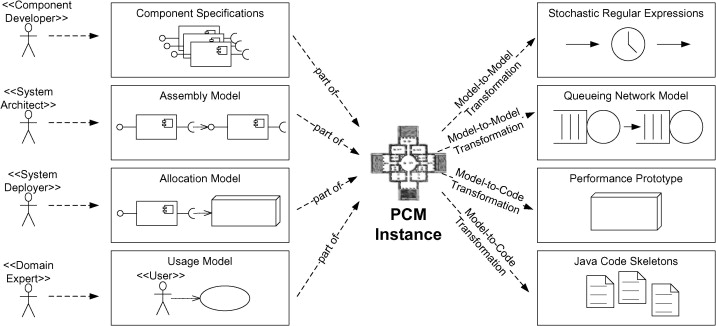
\includegraphics[width=15cm]{palladio-cbse-process}
  \caption{\small{Instancia de un modelo PCM. Tomado de \cite{happe-et-al}}}
  \label{fig:pcm-instance}
\end{figure}

\begin{itemize}
    \item \textbf{Especificaciones de componentes} son descripciones abstractas y paramétricas de los componentes de software. En las especificaciones de software se proporciona una descripción del comportamiento interno del componente así como las demandas de sus recursos en RDSEFFs (\emph{Resource Demanding Service EFFect specifications}) utilizando una sintaxis similar a los diagramas de actividad de UML.
    \item \textbf{Un modelo de ensamblaje} (\emph{assembly model}) especifica qué tipo de componentes se utilizan en una instancia de aplicación modelada y si las instancias del componente se replican. Además, define cómo las instancias del componente se conectan representando la arquitectura de software.
    \item El entorno de ejecución y los recursos, así como el despliegue (\emph{deployment}) de instancias de componentes para dichos contenedores de recursos se definen en un \textbf{modelo de asignación} (\emph{allocation model}).
    \item El \textbf{modelo del uso} especifica la interacción de los usuarios con el sistema utilizando una sintaxis similar al diagrama de actividades de UML proporcionando una descripción abstracta de la secuencia y la frencuencia en que los usuarios activan las operaciones disponibles en un sistema.
\end{itemize}

Un modelo PCM abstrae un sistema de software a nivel de arquitectura y se anota con consumos de recursos que fueron medidos previamente u otros que son estimados. El modelo puede entonces ser usado en transformaciones de modelo-a-modelo o modelo-a-texto a un modelo de análisis en particular (redes de colas o simulación de código) que puede ser analíticamente resuelto o simulado para obtener resultados sobre el rendimiento y predicciones del sistema modelado. Los resultados del rendimiento y las predicciones pueden ser utilizadas como retroalimentación para evaluar y mejorar el diseño inicial, permitiendo así una evaluación de calidad de los sistemas de software en base a un modelo\cite{noorshams}. 

\subsection{Retos de investigación asociados a Ingeniería de rendimiento}
Informes recientes como \cite{microservices-challenges} y \cite{performance-devops} señalan que los principales retos en investigación de ingeniería de rendimiento en la actualidad están asociados con generación de modelos a partir de código, integración de la evaluación de rendimiento en el ciclo de desarrollo y modelado de rendimiento de sistemas en la nube.

Con respecto a integración en ciclos de desarrollo de software y principalmente en aquellos basados en DevOps, una tendencia hacia una estrecha integración entre equipos desarrollo y operaciones, en \cite{performance-devops} se destaca que la necesidad de tal integración está orientada por el requerimiento de adaptar aplicaciones empresariales a los cambios del ambiente del negocio continuamente. El rendimiento describe las propiedades del sistema con respecto a su ejecución y uso de recursos. Métricas comunes son tiempo de respuesta, \emph{throughput} y la utilización de los recursos. Los objetivos de rendimiento para aplicaciones empresariales son típicamente definidos al establecer cotas superiores/inferiores para estas métricas y transacciones de negocio específicas. 

\subsubsection{Actividades de administración del rendimiento}
Evaluación del rendimiento basado en modelos:
\begin{itemize}
    \item La representación de la memoria principal y del recolector de basura aún no están explícitamente integrados ni considerados en los modelos de rendimiento
    \item La selección de técnicas apropiadas de solución requiere de mucha experiencia
\end{itemize}

Extracción de modelos de rendimiento y de cargas de trabajo:
\begin{itemize}
    \item La precisión de los modelos puede llegar a expirar si no son actualizados cuando hay cambios. Mecanismos de detección son requeridos para aprender cuando los modelos son antiguos y hay que actualizarlos.
    \item La extracción de capacidades de rendimiento se basa en una combinación de software y los recursos de hardware en los que se implementa. Este enfoque combinado es compatible con la precisión de la predicción, pero está menos calificado con respecto a la portabilidad de los conocimientos a otras plataformas. Una dirección de investigación futura podría ser extraer modelos separados (por ejemplo, \emph{middleware} y modelos de aplicación separados). 
\end{itemize}

\subsubsection{Modelos de rendimiento durante etapas diseño }
\begin{itemize}
    \item Los retos de utilizar modelos de rendimiento en etapas tempranas de desarrollo es que usualmente es difícil validar la precisión de los modelos hasta que un sistema en ejecución exista. Las predicciones de rendimiento basadas en suposiciones, entrevistas y pruebas previas pueden ser también imprecisas y por tanto las decisiones que se hagan a partir de estas predicciones.
\end{itemize}

En relación con sistemas y arquitecturas en la nube como las basadas en microservicios otras tecnologías importantes para \emph{deployment} como, virtualización basada en contenedores y soluciones de orquestación de contenedores han emergido. Estas tecnologías permiten explotar plataformas en la nube, proporcionando altos niveles de escalabilidad, disponibilidad y portabilidad para microservicios. A pesar del hecho de que es una necesidad inherente contar con escalabilidad y elasticidad, la ingeniería de rendimiento para microservicios hasta ahora ha tenido poca atención por parte de las comunidades tanto de microservicios como de comunidades de investigación de ingeniería de rendimiento\cite{microservices-challenges}. Un gran cuerpo de conocimiento y buenas prácticas para ingeniería de rendimiento para desarrollo tradicional de software y arquitecturas está disponible. Sin embargo, sus aplicaciones en DevOps imponen tanto retos como oportunidades.

\subsection{Retos de investigación en microservicios}

Pruebas de rendimiento
\begin{itemize}
    \item Reemplazar y compensar pruebas extensivas de integración y de sistema por un control detallado de los entornos de producción
    \item Alinear las pruebas de rendimiento y pruebas de regresión de rendimiento con prácticas de entrega continua, por ejemplo, acelerar las estas de pruebas correspondientes.
    \item Selección dinámica y semi automática de pruebas de rendimiento
\end{itemize}

Monitoreo
\begin{itemize}
    \item Instrumentación para monitoreo distribuido arquitecturas microservicios políglotas 
    \item Métricas adicionales para monitorear microservicios
    \item Técnicas de detección precisa de anomalías en arquitecturas de microservicios
\end{itemize}


Modelado del rendimiento: de momento no existen enfoques para modelado del rendimiento de microservicios 
\begin{itemize}
    \item Adoptar modelos de rendimiento para casos de uso como planeamiento de capacidad, confiabilidad y resiliencia
    \item Buscar abstracciones de modelado apropiadas 
    \item Extracción automática de modelos de rendimiento
    \item Aprender del comportamiento de la infraestructura e integrarlo en los modelos de rendimiento
\end{itemize}




\subsection{Herramientas para modelaje de rendimiento de software}
En \cite{thijmen-thesis} se llevó a cabo un extensa encuesta sobre el estado del arte de herramientas de modelado de rendimiento de software. Como resultado, se lograron identificar varias herramientas para construir modelos de rendimiento pero, a pesar de esto, muchas de ellas fueron consideradas como no-maduras de acuerdo a los criterios de selección aplicados.

Primero, la herramienta debería de demostrar que se puede aplicar para el modelado de arquitecturas de software, este criterio excluyó a muchas herramientas de bajo nivel. Segundo, debe de estar liberada y disponible y esto excluyó a muchas herramientas descritas en artículos de investigación. Por último, debe ser madura y medianamente estable y este fue requerimiento que no cumplieron mucha de las herramientas publicadas en artículos de investigación.

Al final, se seleccionarion seis herramientas que se consideraron suficientemente maduras y promisorias las cuales se podrían ajustar para abordar problemas de modelado de arquitecturas. 

\paragraph{1. Java Modeling Tools (JMT):} es un conjunto de programas en Java que apoyan el modelado y análisis de modelos de redes de colas. Dentro de las ventajas que tiene es que puede obtener soluciones computacionalmente baratas de modelos de redes de colas. También cuenta con una extensa interfaz gráfica de usuario que ayuda a los usuarios a través del proceso de modelado y análisis, esto baja su curva de aprendizaje. Una de sus limitaciones es que se ha señalado que es desafiante modelar sistemas de software industrial usando un formalismos simples de modelos de redes de colas. La herramienta se encuentra disponible en \url{http://jmt.sourceforge.net}.

\paragraph{2. Layered Queueing Network Solver (LQNS):} es una herramienta de redes de colas(LQN por sus siglas en inglés) en capas y tiene el conjunto de características más completo de varias herramientas de LQN en capas comunes. Las LQNs ofrecen una forma fácil de expresar el uso de los recursos y encontrar cuellos de botella en servidores. Los algoritmos de análisis para LQN pueden escalar a sistemas grandes y puede ser usados para modelar grandes cantidades de solicitudes concurrentes. Dentro de sus limitaciones se menciona el hecho que LQN son menos adecuadas para modelar restricciones de tamaño de memoria que los modelos de redes de colas. De igual forma, en su manual de usuario se listan una serie de defectos conocidos y pocos detalles sobre estos son proporcionados. La herramienta se encuentra en \url{http://www.sce.carleton.ca/rads/lqns/}.

\paragraph{3. Palladio-Bench:} implementa el \emph{Palladio Component Model}. El software se encuentra disponible como un \emph{plug-in} de Eclipse IDE y puede ser obtenido en el sitio Web \url{http://www.palladio-simulator.com/}. Esta herramienta puede ahorrar tiempo cuando se modelan componentes que son reutilizados en otros modelos. Es posible especificar las demandas de recursos dependientes de la entrada, probabilidades condicionales y contadores de iteraciones. Por ejemplo, el tiempo de ejecución de un componente puede hacerse dependiente del tamaño del archivo que va a procesar. Las limitaciones que se han reportado de esta herramienta incluyen poco soporte para concurrencia y del modelado del ambiente de ejecución. 

\paragraph{4. Möbius:} es una herramienta que implementa múltiples lenguajes de modelado y inclusive permite combinarlos para explotar su expresividad o para combinar múltiples aspectos de un sistema dentro de un modelo. Dentro de los lenguajes de modelaje ofrecidos, el SAN, \emph{Buckets and Balls} y PEPA puede ser utilizados para modelado de rendimiento. Varios de los formalismos soportados por Möbius se basan en cadenas de Markov y por lo tanto sufren del problema de explosión espacial del estado. Puede haber una reducción en el número de estados de uno a dos órdenes de magnitud utilizando técnicas de agrupamiento, pero lo que esto significa en la práctica aún no está claro. La página Web de la herramienta es \url{https://www.mobius.illinois.edu/}

\paragraph{5. SPE-ED:} implementa el enfoque SPE documentado por Smith y Williams\cite{spe-ed}. Es una de las herramientas más maduras que se adecua a la predicción temprana del rendimiento. Utiliza modelos simples y que son fáciles de construir y resolver. SPE-ED solamente soporta redes de tipo $M/M/n$, lo que significa que los tiempos de llegada y servicio solamente pueden ser modelar teniendo distribuciones exponenciales. También se menciona que SPE-ED reporta solamente tiempos medios, lo cual es una limitación importante para alguien que quiera basar sus decisiones en valores extremos. SPE-ED se puede encontrar en \url{http://www.spe-ed.com}.

\paragraph{6. QPME:} De acuerdo con el sitio Web \emph{Petri Nets World}\footnote{\url{http://www.informatik.uni-hamburg.de/TGI/PetriNets/tools/quick.html}} QPME es una de las pocas herramientas de redes de Petri que sportan análisis de rendimiento avanzado y es la única herramienta actual que soporta redes de colas de Petri jerárquicas. El formalismo de modelado de redes de colas de Petri ha demostrado ser muy adecuado para representar sistemas de comercio electrónico distribuidos pero, por la falta de buenas herramientas es que el desarrollo de QPME fue motivado. QPME se ocupa de reducir el problema de explosión del espacio de estado. Se señala que con QPME no se puede modelar restricciones de memoria y que de momento no hay técnicas de análisis disponible, solamente de simulación. Otra limitación es que solamente se puede modelar llamadas sincrónicas y esto no lo hace adecuado para modelar sistemas de paso de mensajes. QPME se puede encontrar en \url{https://se.informatik.uni-wuerzburg.de/tools/qpme/}.

%---
%
%
%Un atributo no funcional que es usualmente es de alta importancia durante el desarrollo de software es el rendimiento del sistema en cuestión. Si los sistemas sufren de un rendimiento insuficiente, esto hace que usualmente no se utilicen como se esperaba o bien hacen que los proyectos fallen. Por lo tanto, la predicción del rendimiento de los sistemas de software está en el centro de agendas de investigación desde finales de los años noventa\cite{huber-et-al}. El término rendimiento a menudo  caracteriza el comportamiento en el tiempo y la eficiencia de los recursos de los sistema de hardware y de software. Las propiedades de rendimiento más importantes son tiempos de respuesta, \emph{throughput} y utilización de recursos.
%
%La ingeniería de rendimiento de software se dedica a evaluar el rendimiento de sistemas de software al ofrecer diferentes métodos como modelado analítico, simulación y toma de mediciones. El objetivo de SPE es conducir evaluaciones del rendimiento de arquitecturas de software tan pronto como se pueda. 
%
%En SPE, la creación y evaluación de modelos de rendimiento es un concepto clave para evaluar cuantitativamente el rendimiento del diseño de un sistema y predecir el rendimiento de otras alternativas de diseño. Un modelo de rendimiento captura el comportamiento relevante al rendimiento de un sistema para identificar el efecto de cambios en la configuración o en la carga de trabajo en el rendimiento. Permite predecir los efectos de tales cambios sin necesidad de implementarlo y ponerlo en producción, que podrían ser no solamente tareas costosas sino también un desperdicio en el caso que un el hardware con el que se cuenta pruebe ser insuficiente para soportar la intensidad de la carga de trabajo.
%
%El punto de inicio de la mayoría de enfoques de SPE es la arquitectura del sistema de software. La arquitectura puede ser mejorada con anotaciones de rendimiento. Este modelo de software debe ser transformado en un modelo de rendimiento --como por ejemplo redes de colas, redes de Petri o cadenas de Markov -- para luego ser resuelto para las métricas de interés.
%
%En el área de SPE, la idea de usar tecnologías orientadas a modelos ha ganado atención porque estas proporcionan transformación automática desde algún origen hacia un modelo de rendimiento. Sin embargo, los métodos de predicción de rendimiento basados en modelos requieren meta-modelos adecuados. Estos meta-modelos formalizan la sintáxis y semántica del modelo origen y destino. La transformación y procesamiento automático simplifica el enfoque de ingeniería de rendimiento de software y lo hace menos propenso a errores.
%
%\subsection{Predicción de rendimiento dirigida por modelos}
%La predicción del rendimiento dirigida por modelos permite a los arquitectos de software especificar modelos de rendimiento en un lenguaje especifico a su dominio. Esto puede a partir de modelos UML anotados con información relevante al rendimiento o por medio de lenguajes de descripción de arquitecturas especializados para la predicción de rendimiento como \emph{Palladio Component Model} (PCM) \cite{palladio-seminal, palladio-blue-book}. Para derivar métricas de rendimiento, el modelo de software se transforma en un modelo de rendimiento, como se muestra en la figura \ref{fig:model-driven-performance-prediction}. Las métricas de rendimiento derivadas del modelo de rendimiento deberían traducirse nuevamente al modelo de diseño, para permitir una interpretación fácil para los arquitectos de software.






\subsection{\emph{Middleware} Orientado a Mensajes} \label{sec:mom}

Junto con el crecimiento de Internet, los sistemas distribuidos han crecido a una escala masiva. Hoy en día, estos sistemas puede involucrar a miles de entidades distruidas globalmente. Esto ha motivado el estudio de modelos de comunicación y sistemas flexibles, que puedan reflejar la naturaleza dinámica y desacoplada de las aplicaciones.

La integración de tecnologías heterogéneas es una de las áreas principales en donde la comunicación basada en mensajes juega un papel clave. Más y más compañías se enfrentan al problema de integrar sistemas y aplicaciones heterogéneas dentro y fuera de la organización ya sea por fusiones, adquisiciones, requisitos comerciales o simplemente un cambio en la direción tecnológica. No es raro encontrar una gran cantidad de tecnologías y plataformas dentro de una solo compañía, desde productos de código libre y comerciales hasta sistemas y equipos heredados (\emph{legacy}).

La comunicación basada en mensajes también ofrece la habilidad de procesar solicitudes de manera asincrónica, proporcionando a los arquitectos y desarrolladores soluciones para reducir o eliminar cuellos de botella en un sistema e incrementar la productividad del usuario final y del sistema en general. Dado que la comunicación basada en mensajes provee un alto grado de desacoplamiento entre componentes, los sistemas que utilizan esta tecnología también logran contar con altos grados de agilidad y flexibilidad en su arquitectura.

A los sistemas de mensajería de aplicación-a-aplicación que se utilizan sistemas de negocios se les denomina genéricamente sistemas de mensajería empresarial o \emph{middleware} orientado a mensajes\cite{jms20}. MOM permite a dos o más aplicaciones intercambiar información en forma de mensajes. Un mensaje, en este caso, es un paquete autocontenido de datos de negocio y encabezados de enrutamiento de red. Los datos de negocio contenidos en un mensaje puede ser cualquier cosa, van a depender de cada negocio, y usualmente contiene información acerca de algún tipo de transacción. En sistemas de mensajería empresariales, los mensajes informan a una aplicación de la ocurrencia de algún evento en otro sistema. La tasa de mensajes depende de la capacidad de la implementación de MOM o \emph{broker}. El retraso depende de la latencia en el \emph{broker} y en los caminos de entrada y salida\cite{chew}.

Al usar MOM, los mensajes son trasmitidos desde una aplicación a otra a través de la red. Productos de \emph{middleware} empresarial aseguran que los mensajes se distribuyan correctamente entre las aplicaciones. Además estos productos usualmente proporcionan tolerancia a fallos, balanceo de carga, escalabilidad y soporte transaccional para sistemas que necesitan que necesitan intercambiar de manera confiable grandes cantidades de mensajes.

Los fabricantes de MOM usan diferentes formatos de mensajes y protocolos de red para intercambiar mensajes pero la semántica básica es la misma. Una interfaz de programación de aplicación (API, por sus siglas en inglés) se utiliza para crear un mensaje, cargar los datos, asignar información de enrutamiento y enviar el mensaje. La misma API se utiliza para recibir los mensajes producidos por otras aplicaciones.

En todos los sistemas modernos de mensajería empresarial, las aplicaiones intercambian mensajes a través de canales virtuales llamados destinos(\emph{destinations}). Cuando un mensaje se envía, se dirije a un destino (por ejemplo una cola o un tópico) no a una aplicación específica. Cualquier aplicación qu subscriba o registre un interés en ese destino puede recibir el mensaje. De esta forma, las aplicaciones que reciben mensajes y aquellas que envían mensajes están desacopladas. Los emisores y receptores no están enlazados uno con otro de ninguna forma y pueden enviar y recibir mensajes como mejor les parezca.

Un concepto clave de MOM es que los mensajes son entregados de forma asincrónica desde un sistema a otros sobre la red. El entregar un mensaje de manera asicrónica significa que el emisor no requiere esperar a que el mensaje sea recibido o manejado por el receptor, él es libre de enviar el mensaje y continuar su procesamiento. Los mensajes asicrónicos son tratados como unidades autónomas: cada mensaje es autocontenido y lleva consigo todos los datos necesarios para ser procesado.

En comunicación de mensajes asincrónicos, las aplicaciones usan una API para contruir un mensaje, luego pasarlos al MOM para su entrega a uno o varios recipientes (Figura \ref{fig:mom}). Un mensaje es un paquete de datos que es enviado desde una aplicación a otra sobre la red. El mensaje debe de ser autodescriptivo en el sentido que debe de contener todo el contexto necesario para que permit a los recipientes llevar a cabo su trabajo de forma independiente. 


\begin{figure}[h]
  \centering
  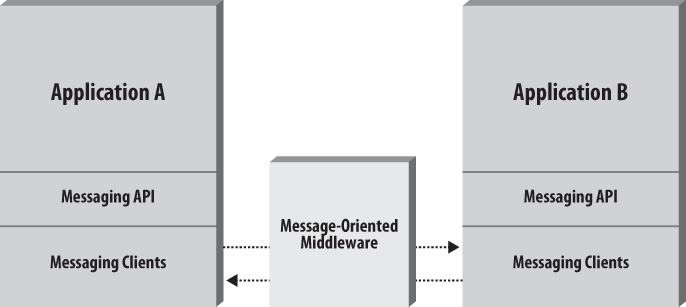
\includegraphics[width=10cm]{jms20-mom}
  \caption{\small{\emph{Middleware} Orientado a Mensajes. Tomado de \cite{jms20}}}
  \label{fig:mom}
\end{figure} 

La arquitecturas de MOM de hoy en día varían en su implementación. Van desde las arquitecturas centralizadas que dependen de un servidor de mensajes para realizar enrutamiento a arquitecturas descentralizadas que distribuyen el procesamiento del servidor hacia los clientes. Una variedad de protocolos como \texttt{TCP/IP, HTTP, SSL} y \texttt{IP} son empleados como capa de transporte de red.

Los sistemas de mensajería están compuestos por clientes de mensajería (\emph{messaging clients}) y algún tipo de servidor MOM. Los clientes envían mensajes al servidor de mensajería el cual distribuye estos mensajes a otros clientes. El cliente es una aplicación de negocio o componente que es usa una API de mensajería.

\subsection{Modelos de mensajería}

\subsubsection{Punto-a-Punto}
Este modelo de mensajería permite a los clientes enviar y recibir mensajes de forma síncrona como asíncrona a través de canales virtuales conocidos como colas. En este modelo a los productores de mensajes se les llama emisores (\emph{senders}) y a los consumidores se les conoce como receptores (\emph{receivers}). El modelo punto-a-punto ha sido tradicionalmente un modelo basado en \emph{polling}, en donde los mensajes son solicitados desde la cola en lugar de ser puestos en el cliente automáticamente. Los mensajes que se envían a una cola son recibidos por uno y solo un \emph{receiver}, aunque pueden haber otros \emph{receivers} escuchando en la cola por el mismo mensaje. Este es un modelo que promueve acoplamiento esto porque generalmente el \emph{sender} conocer cómo el mensaje va a ser utilizado y quién lo va a recibir. 

\subsubsection{\emph{Publish-and-Subscribe}}
En este modelo, los mensajes son publicados en un canal virtual llamado tópico. Los productores de mensajes son conocidos como \emph{publishers} y a los consumidores se les llama \emph{subscribers}. Los mensajes pueden ser recibidios por múltiples \emph{subscribers}, a diferencia del modelo punto-a-punto. Cada \emph{subscriber} recibe una copia de cada mensaje. Este es un modelo basado en \emph{push} en donde los mensajes son automáticamente transmitidos a los consumidores sin que estos tengan que solicitarlos o revisar la cola por nuevos mensajes. 

Este modelo tiende a ser menos acoplado que el modelo punto-a-punto debido a que el publicador del mensaje generalmente no está conciente de cuántos subscritores hay y lo qué van a hacer estos con el mensaje.


\begin{figure}[h]
  \centering
  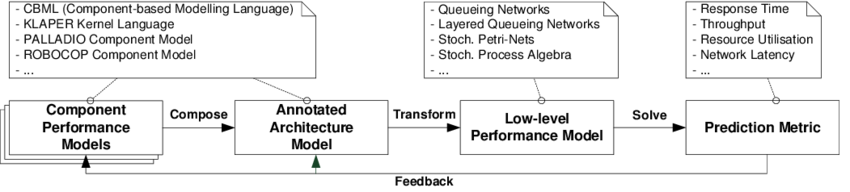
\includegraphics[width=15cm]{model-driven-performance-prediction}
  \caption{\small{Predicción de rendimiento dirigido por modelos. Tomado de \cite{happe-et-al}}}
  \label{fig:model-driven-performance-prediction}
\end{figure}


\subsection{Enfoques de ingeniería de rendimiento para \emph{middleware} orientado a mensajes}
En \cite{happe-et-al} se extiende el \emph{Palladio Component Model} con \emph{performance completions} para \emph{middleware} orientado a mensajes. \emph{Performance completions}\cite{woodside-et-al-2} proporcionan el concepto general de incluir detalles de bajo nivel de ambientes de ejecución en modelos de rendimiento. Con la extensión del modelo, los arquitectos de software puede especificar y configurar comunicación basada en mensajes utilizando un lenguaje basado en patrones de mensajería.

La influencia en el rendimiento de \emph{middleware} orientado a mensajes fue estudiada en \cite{liu-gordon}. Se consideró el \emph{middleware} como un factor determinante del rendimiento en sistemas distribuidos y se hizo un mayor enfoque en su modelado y evaluación. Se propuso un enfoque basado en medición en combinación con modelos matemáticos para predecir el rendimiento de aplicaciones J2EE\footnote{\emph{Java Enterprise Edition}}. Las mediciones proporcionan los datos necesarios para calcular los valores de entrada del modelo de red de cola. El cálculo refleja el comportamiento de la aplicación en particular. La red de cola se resuelve para derivar métricas de rendimiento tales como tiempos de respuesta y \emph{throughput} de la aplicación. 

La investigación llevada a cabo en \cite{chew} presenta un modelo abstracto de \emph{middleware} orientado a mensajes basado en Apache Qpid junto con el uso de modelos exógenos de autorregressión (ARX por sus siglas en inglés) que describen el comportamiento del \emph{middleware} durante condiciones de cuellos de botella. Los modelos ARX son modelos autorregresivos en donde la salida depende de la salida anterior así como de estimulos externos. Estos componentes son integrados para producir una técnica generalizada de calibración para rendimiento del \emph{middleware} y detección de cuellos de botella en el mismo.

En \cite{martince-et-al} se construyen modelos de rendimiento para \emph{middleware} que implementa el estándar \emph{Java Messaging Service} (JMS). Se utiliza análisis de código y mediciones experimentales de implementaciones de JMS populares para mostrar situaciones en las que el rendimiento observado no es predecido de forma preciesa por otros modelos. Se proporciona un análisis técnico detallado de los efectos observados como base esencial para futuros trabajos de modelado. Por último, se diseña un modelo de rendimiento que captura estos efectos y se valida el modelo utilizando mediciones experimentales.

Un un modelo analítico $M/M/1$ con políticas\emph{first in - first out} y prioridad de colas fue diseñado y desarrolloado en \cite{alwakeel} para evaluar el rendimiento de \emph{middleware} orientado a mensajes y llamados a procedimientos remotos (RPC por sus siglas en inglés). Los modelos comparan el rendimiento de \emph{middleware} orientado a mensajes y RPC con prioridad de colas y analizan el \emph{throughput} de estos paradigmas de comunicación. Varios parámetros de entrada son usados para determinar la configuración óptima para lograr el máximo rendimiento. Los resultados prueban que al utilizar \emph{middleware} orientado a mensajes con prioridad de cola, el \emph{throughput} del sistema puede ser mejorado. 

\subsection{Posicionamiento de la investigación con respecto a la literatura consultada}
A partir de lo recolectado se pudo conocer que mucho del esfuerzo que se ha hecho en este campo de estudio ha tenido baja aceptación en la industria pero que, por otro lado, compañías y sistemas que han utilizado estos métodos de modelaje y evaluación han obtenido buenos resultados. Queda claro también que la aplicación de estos modelos permiten entender la influencia que tienen tanto de los diferentes componentes de software como el impacto que pudiera generar en ellos durante la ejecución de un sistema.

También se pudo reconocer que existe necesidad en aplicar enfoques de modelado del rendimiento en el desarrollo de sistemas modernos. No existen enfoques de modelado de rendimiento para microservicios que hoy en día es un estilo de arquitectura de software sumamente popular. Es por esto que se considera que la realización de estudios exploratorios para determinar la influencia en el rendimiento que tienen diferentes componentes, librerías y productos de software sobre un sistema van a brindar nuevo conocimiento para dar a conocer factores que favoren o desfavorecen el uso de los mismos y, además de esto, podría representar un marco de referencia inicial por medio del cual se pueda evaluar la adopción de estas tecnologías \emph{a priori}. 

Por último, durante la búsqueda de artículos se encontraron muy pocos de ellos provenientes de universidades de latinoamérica. Esto representa, a juicio del autor, una oportunidad para estudiar, probar y generar conocimiento sobre estos temas.  

\newpage
\section{Aplicación de referencia} \label{ch:aplicacion-referencia}

Durante la elaboración de la revisión de la literatura, se procedió a estudiar algunas de las aplicaciones que se utilizaron en la realización de los respectivos estudios con el fin de tomar alguno de estos como referencia para la investigación propuesta. Para seleccionar una aplicación que se adecue al tema propuesto, se establecieron los siguientes criterios:
\begin{enumerate}
    \item Aplicación de código libre
    \item Que cuente con modelos de rendimiento hechos en \emph{Palladio Workbench}
    \item Desarrollada en un lenguaje de programación y con herramientas de actualidad
    \item Que continue siendo mantenida y mejorada por sus autores
\end{enumerate}


Del listado anterior, quizás el criterio más restrictivo es el \#2 pero al mismo tiempo se considera el de mayor importancia debido a que en esta investigación se están dando los primeros pasos con el modelado de arquitecturas utilizando Palladio y no se deseaba empezar desde cero sino más bien tomar un modelo de referencia e ir haciendo pequeñas modificaciones y probar los resultados.

Durante la exploración de aplicaciones candidatas se pudo constatar que muchas de ellas fueron creadas para probar los objetivos de un estudio en particular y luego cayeron en desuso. A pesar que varias de ella se pueden acceder fácilmente por medio de Internet, carecen de mantenimiento y documentación y esto causa que sean difíciles de evaluar. Una de las motivaciones principales detrás de la elección de método Palladio para modelado de arquitecturas de software, es que este hay sido un proyecto que cuenta con un nivel de madurez importante y está en constante mantenimiento y mejora por parte de su equipo de desarrollo. Aún así se pudo encontrar aplicaciones que utilizaron modelos de Palladio pero se encontraban en ``abandono''. 

\emph{CloudScale}, un proyecto generado a partir de la experiencia de Palladio, es un método que permite identificar y gradualmente resolver problemas de escalabilidad en aplicaciones existentes. \emph{CloudScale} también permite modelar alternativas de diseño y el análisis de su efecto en la escalibilidad y costo\cite{cloudscale}. El sitio Web de \emph{CloudScale}, \url{http://www.cloudscale-project.eu/} contiene publicaciones e información general acerca de este método, así también como del \emph{CloudScale Environment}, un entorno de desarrollo integrado creado para modelaje y análisis. 

Con el fin de validar \emph{CloudScale}, varias aplicaciones fueron creadas. Una ventaja de las aplicaciones que utlizan \emph{CloudScale} es que deben de tener un modelo basado en Palladio para su posterior procesamiento. Otra de las cosas que hicieron que las aplicaciones creadas para esta metología resultaran atractivas para esta investigación, es que el proyecto \emph{CloudScale} es reciente por lo que estas aplicaciones no se consideran como ``viejas'' y se les da mantenimiento. 

Una de estas aplicaciones que se crearon para probar esta metolodología es \emph{CloudStore}, una aplicación Web de código libre que emula una tienda (\emph{e-commerce}) de libros en línea. Su objetivo principal es ser utilizada para el análisis de las características de los sistemas en la nube como escalabilidad, capacidad, elasticidad y eficiencia. Fue desarrollada como la aplicación de muestra para validar las herramientas de \emph{CloudScale}.

La aplicación fue desarrollada en Java utilizando la librerías de \emph{Spring} y se ejecuta en un servidor Tomcat. Utiliza una base de datos MySQL. Para mayor información sobre \emph{CloudStore}, se puede visitar su repositorio en GitHub: \url{https://github.com/CloudScale-Project/CloudStore}.

\begin{figure}[h]
  \centering
  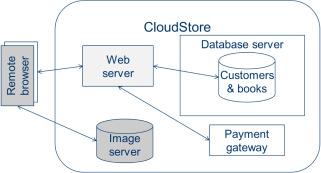
\includegraphics[width=10cm]{conceptual-cloudstore-architecture}
  \caption{\small{Arquitectura Conceptual de CloudStore. Tomado de \cite{happe-et-al}}}
  \label{fig:cloudstore-conceptual}
\end{figure}

En la figura \ref{fig:cloudstore-conceptual} se muestra la arquitectura conceptual de \emph{CloudStore}. Tiene un diseño simple: una aplicación Java que se ejecuta en un servidor Web y que realiza consultas a una base de datos MySQL. Para llevar a cabo los pagos, la aplicación se comunica con un \emph{gateway} para pagos, un servicio Web publicado en un servidor externo al del \emph{CloudStore} que simula el tiempo de respuesta de podría tomar realizar un pago.

Una característica de \emph{CloudStore} particularmente atractiva para este estudio es precisamente el \emph{gateway} de pagos. La interacción entre \emph{CloudStore} y este \emph{gateway} de pagos representa un clásico escenario de integración de sistemas. En su versión original, \emph{CloudStore} realiza llamadas a este \emph{gateway} de pagos de manera \emph{ad hoc} y es aquí en donde la introducción de comunicación basada en mensajes puede ser una mejor opción al actual debido que:
\begin{itemize}
    \item Permite que \emph{CloudStore} se desacople del \emph{gateway} de pagos: la aplicación no necesita saber información específica de este \emph{gateway} ni la forma en cómo debe interactuar con él, esto se lo delega a un tercero. 
    \item La comunicación basada en mensajes puede garantizar el envío de peticiones al gateway de pagos.
\end{itemize}


\subsection{Adaptación de \emph{CloudStore}}
Con el fin de adaptar \emph{CloudStore} para que soporte comunicación basada en mensajes cuando se ejecute un pago, se propone lo siguiente:
\begin{enumerate}
    \item Selección de una solución para comunicación basada en mensajes
    \item Selección de librería(s) de código para realizar comunicación entre \emph{CloudStore} y la solución seleccionada en el punto anterior
    \item Implementar un consumidor de mensajes de petición de pago: una aplicación que estará monitoreando(\emph{pooling}) y procesando mensajes provenientes de la solución seleccionada en el punto \#1 y que los entregará al \emph{gateway} de pagos. Adicionalmente esta aplicación comunicará al \emph{CloudStore} el estado del procesamiento del pago
    \item Reemplazar el código existente que se dedica a realizar el pago contra el \emph{gateway} de pagos por nuevo código que se comunicará con la solución de mensajería
\end{enumerate}

Para el punto \#1, se seleccionó ActiveMQ\footnote{\url{http://activemq.apache.org/}}, el servidor más popular de mensajería de código libre.
 
Al estar utlizando ActiveMQ, el cual es un servidor que implementa el estándar \emph{Java Messaging Service}, se va a utilizar la librería \texttt{javax.jms} con versión 1.1.

La aplicación consumidora/procesadora de mensajes será una aplicación Java que se va a ejecutar como un servicio. 

\begin{figure}[h]
  \centering
  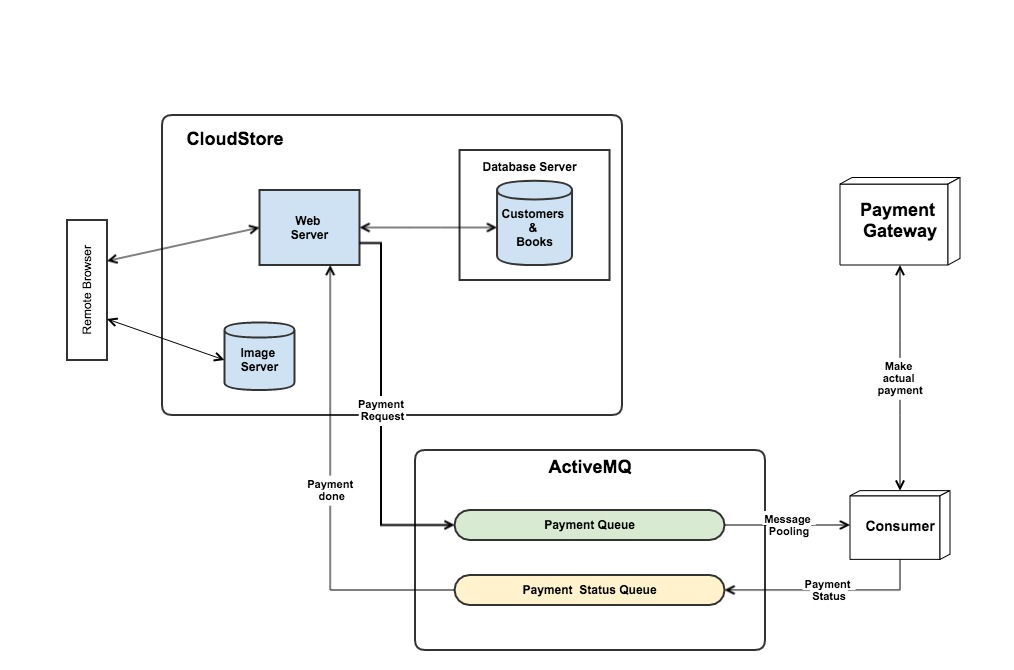
\includegraphics[width=18cm]{cloudstore-jms}
  \caption{\small{Arquitectura Conceptual de CloudStore utilizando comunicación basada en mensajería}}
  \label{fig:cloudstore-jms}
\end{figure}

La arquitectura adaptada de \emph{CloudStore} para que utilice comunicación basada en mensajes se muestra en la figura \ref{fig:cloudstore-jms}. Ahora, en lugar de realizar una llamada \emph{ad hoc} al \emph{gateway} de pagos, la aplicación se comunica con una cola de mensajería para pagos tanto para el envío como para la recepción del pago. A este esquema de comunicación se le conoce como \emph{request-reply}, esto porque la aplicación que inicia la petición se queda a la espera del resultado.

Para realizar un pago, \emph{CloudStore} enviará un mensaje a una cola de pagos, en la figura \ref{fig:cloudstore-jms} se identifica como ``Payment Queue''. La aplicación consumidora de mensajes, estará monitoreando esta cola constantemente con el fin de tomar los mensajes y procesarlos contra el \emph{gateway} de pagos. Una vez que el pago se haya efectuado, la aplicación consumidora envía el resultado del pago a otra cola identificada en la figura \ref{fig:cloudstore-jms} como ``Payment Status Queue''. \emph{CloudStore} estará monitoreando los mensajes provenientes de esta cola con el fin de conocer el estado del pago.

\subsubsection{Aplicación original \emph{vs.} Aplicación modificada}
Para la adaptación de \emph{CloudStore}, se tomó del repositorio de código de este proyecto que se encuentra en \url{https://github.com/CloudScale-Project/CloudStore} y se copió a un nuevo repositorio: \url{https://github.com/tema-selecto-investigacion/cloudstore-boot}. Esto se hizo con el fin de tener mayor control y visibilidad sobre los cambios hechos. En la figura \ref{fig:github-cloudstore-1} se muestra el repositorio creado para \emph{CloudStore}.

Seguidamente, se siguieron las instrucciones para su puesta en ejecución: instalación dependencias de código necesarias y creación de \emph{scripts} para crear la base de datos y agregar registros a la misma. Una vez que la aplicación se construyó y se configuró para que trabajara junto con una base de datos MySQL local, la misma se pudo ejecutar en el puerto \texttt{:8080}.

\begin{figure}[h]
  \centering
  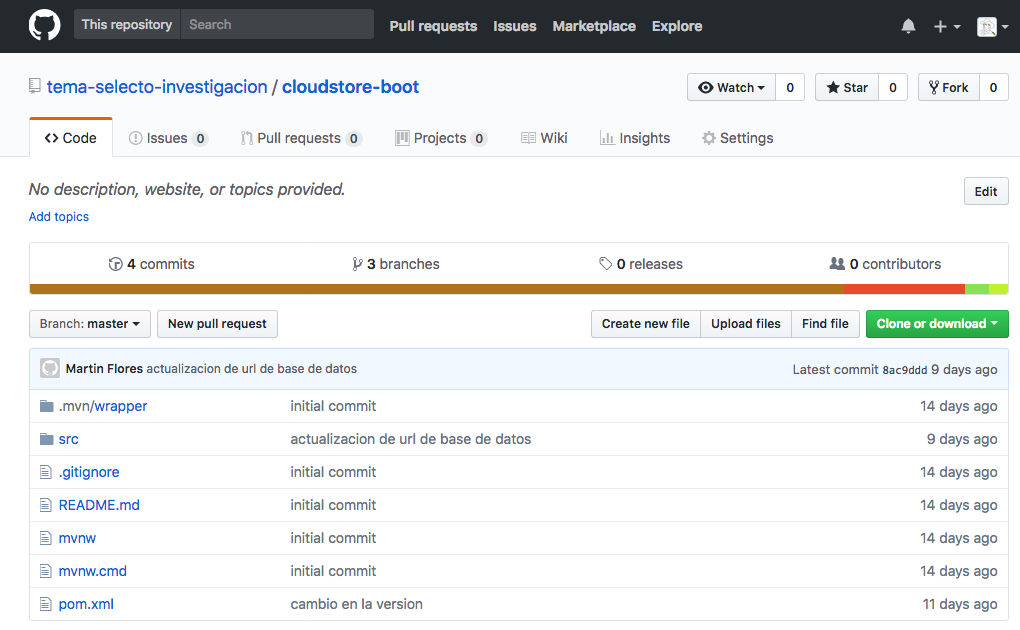
\includegraphics[width=15cm]{github-cloudstore-1}
  \caption{\small{Repositorio de código para CloudStore en GitHub}}
  \label{fig:github-cloudstore-1}
\end{figure}

Luego de ejecutar la aplicación localmente y probar que funcione adecuadamente, se procedió a crear un ambiente de producción en Amazon AWS. Para esto, se creó un ambiente con un servidor Apache Tomcat 8 y una base de datos MySQL utilizando los servicios de \emph{Elastic BeanStalk} y \emph{Relational Database Services}(RDS) respectivamente. A este ambiente se llamó \texttt{cloudstore-plain}. Se configuró la aplicación para que cuando fuera instalada en este ambiente se conectara a la base de datos en AWS.

Cuando ambas, la aplicación local y la instalada en AWS pudieron ser ejecutarse satisfactoriamente, se empezó con la adaptación de \emph{CloudStore}. Lo primero fue instalar e iniciar una instancia de ActiveMQ localmente. En su configuración por defecto, ActiveMQ se ejecuta en el puerto \texttt{:61616} y su aplicación Web de administración en el puerto \texttt{:8161}. Se crearon dos colas de mensajes: \texttt{payment-queue}, en donde se enviarán los mensajes(peticiones) de pago y \texttt{payment-status-queue}, en donde se enviarán los mensajes del estado del pago.  Luego se hizo un nuevo \emph{branch} (rama) en el repositorio de código para los nuevos cambios que se iban a realizar. Este \emph{branch} lleva por nombre \texttt{jms}. Se instaló la dependencia \texttt{javax.jms 1.1} para que la aplicación pudiera comunicarse por medio del estándar \emph{Java Messaging Service}. Se cambió el flujo de trabajo de \emph{CloudStore} para que en lugar de llamar al \emph{gateway} de pago de manera \emph{ad hoc}, se creará un mensaje con la información de la compra para luego enviar este a la cola de mensajes \texttt{payment-queue}. Por último, se agregará código para monitorear y consumir el resultado del pago, el cual debería de ser entregado por la cola \texttt{payment-status-queue}. A este estilo de comunicación se le conoce como \emph{request-reply}: la parte que envia la comunicación debe de aportar algún tipo de encabezado y/o meta-dato al mensaje para su posterior identificación. Luego de enviar el mensaje, la aplicación se pone en modo de monitoreo para filtrar y procesar solamente aquellos mensajes que fueron generados por esta. 

Se creó un nuevo proyecto en Java llamado \texttt{jms-receiver}, cuyo repositorio de código se encuentra en \url{https://github.com/tema-selecto-investigacion/jms-receiver} (Figura \ref{fig:github-jms-receiver}). Este nuevo proyecto va a llevar a cabo las siguientes actividades: monitoreo y consumo constante de mensajes de la cola \texttt{payment-queue}, realizar una llamada al \emph{gateway} de pagos, obtener el resultado del pago y enviarlo por la cola \texttt{payment-status-queue}.

\begin{figure}[h]
  \centering
  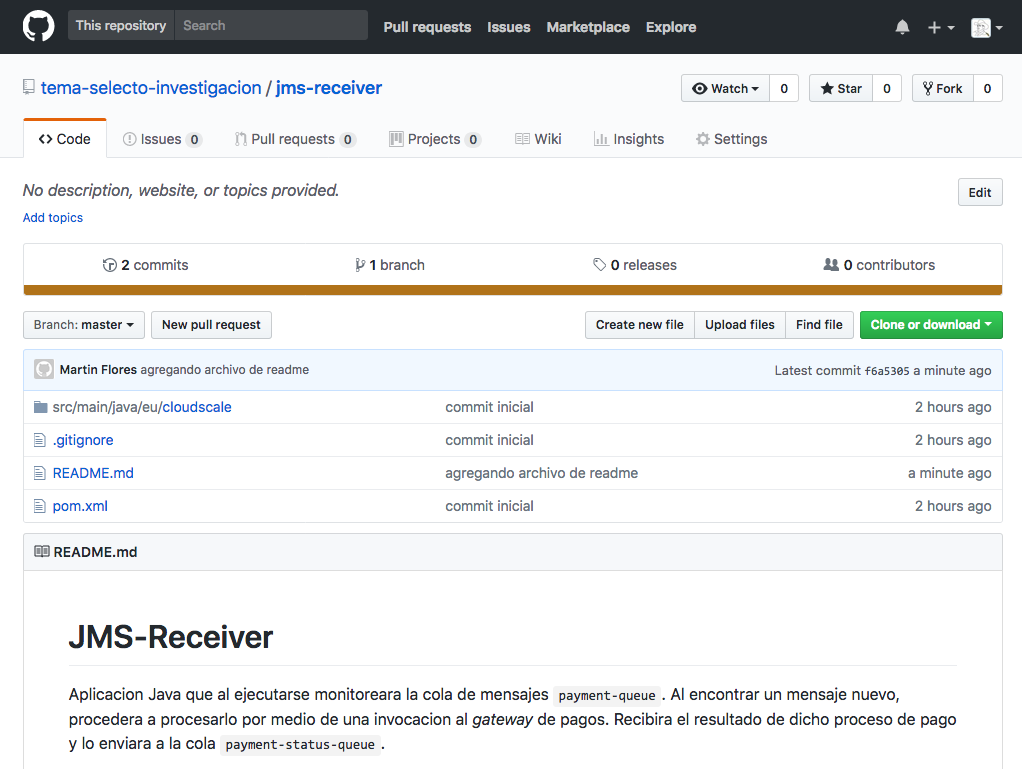
\includegraphics[width=15cm]{github-jms-receiver}
  \caption{\small{Repositorio de código para el proyecto \texttt{JMS-Receiver} en GitHub}}
  \label{fig:github-jms-receiver}
\end{figure}

Primero se probaron los cambios localmente y se pudo comprobar como ahora los mensajes con las peticiones de pagos viajaban a través de las colas de mensajería en lugar de ser generadas a lo interno de \emph{CloudStore}.

Para poner estos nuevos cambios en un ambiente de producción se realizaron las siguientes actividades:
\begin{itemize}
    \item Se creó un nuevo ambiente en \emph{Elastic BeanStalk} llamado \texttt{cloudstore-jms}
    \begin{itemize}
        \item En este nuevo ambiente se va a instalar la aplicación de \emph{CloudStore} modificada que vive en el \emph{branch} \texttt{jms}.
    \end{itemize}

    \item Se provisionó una nueva máquina virtual en el servicio \emph{Amazon Elastic Compute Cloud} (EC2). Una máquina virtual con Ubuntu 16.04, Java y ActiveMQ
    \begin{itemize}
        \item En esta máquina virtual se va a ejecutar la aplicación \texttt{jms-receiver} y el servicio de ActiveMQ con las colas de \texttt{payment-service} y \texttt{paymente-status-queue}
    \end{itemize}
    \item Se configuró la versión de \emph{CloudStore} modificada para que se comunicara con las colas de mensajería que se encuentran en la nueva máquina virtual provisionada
\end{itemize}

Se puede comparar los cambios hechos a la versión original de \emph{CloudStore} en el siguiente \emph{Pull Request}: \url{https://github.com/tema-selecto-investigacion/cloudstore-boot/pull/1}.  

\begin{figure}[h]
  \centering
  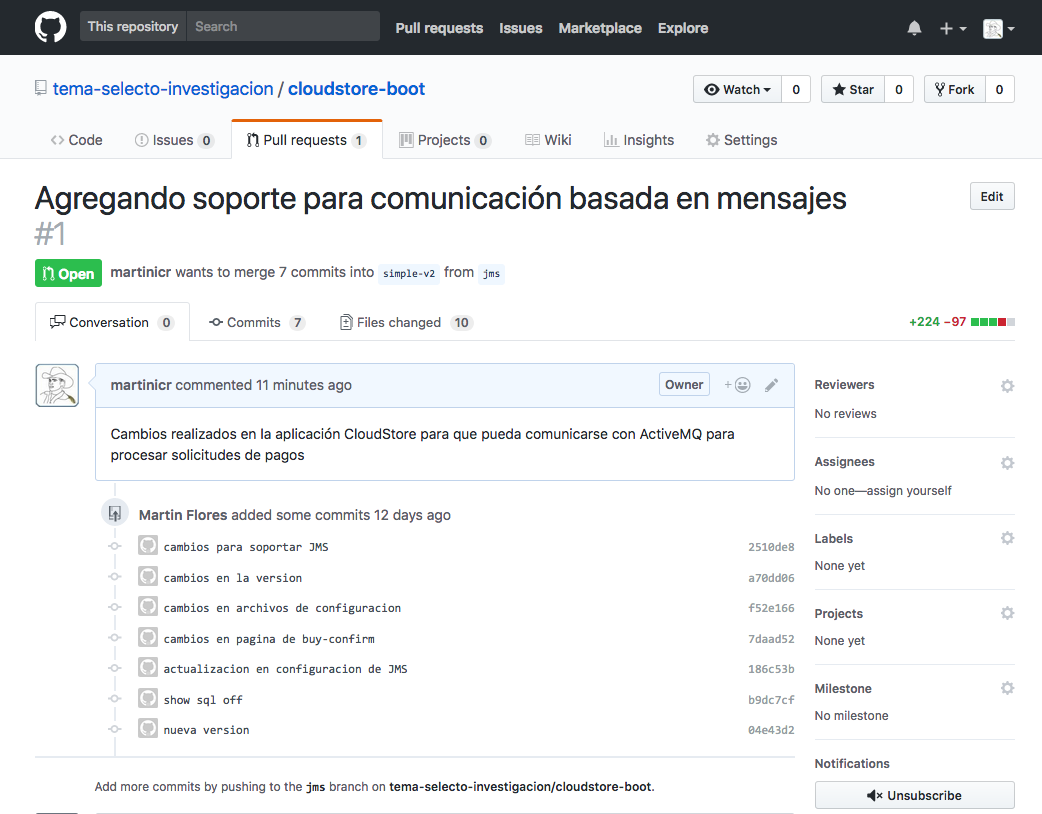
\includegraphics[width=15cm]{github-cloudstore-pr}
  \caption{\small{Diferencias entre el código original de \emph{CloudStore} y el implementado}}
  \label{fig:github-cloudstore-pr}
\end{figure}

En la figura \ref{fig:aws-elb} se pueden ver que los dos ambientes de \emph{CloudStore} se fueron puestos en producción de forma satisfactoria.

\begin{figure}[h]
  \centering
  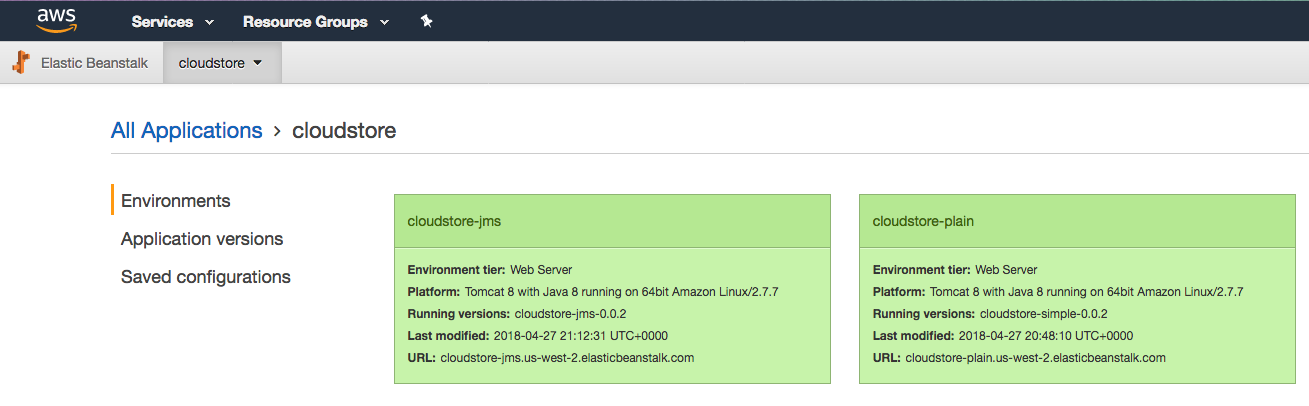
\includegraphics[width=17cm]{aws-elb}
  \caption{\small{Los dos ambientes de \emph{CloudStore} en AWS}}
  \label{fig:aws-elb}
\end{figure}

A continuación se presentan las dos versiones de \emph{CloudStore} ejecutándose en un ambiente de producción. En la figura \ref{fig:aws-cs-plain} se muestra la versión original y el la figura \ref{fig:aws-cs-jms} la versión modificada. Ambas aplicaciones lucen similar, pero apuntan a dominios diferentes y también difieren en la forma en la que se realiza el proceso de pago\footnote{Ambas aplicaciones podrían permanecer no disponibles durante ciertos periódos con el fin de no incurrir en costos innecesarios. En caso de querer probar la aplicación y este no se encuentre disponible, se puede poner en contacto con el autor para su puesta en ejecución.}.

\begin{figure}[h]
  \centering
  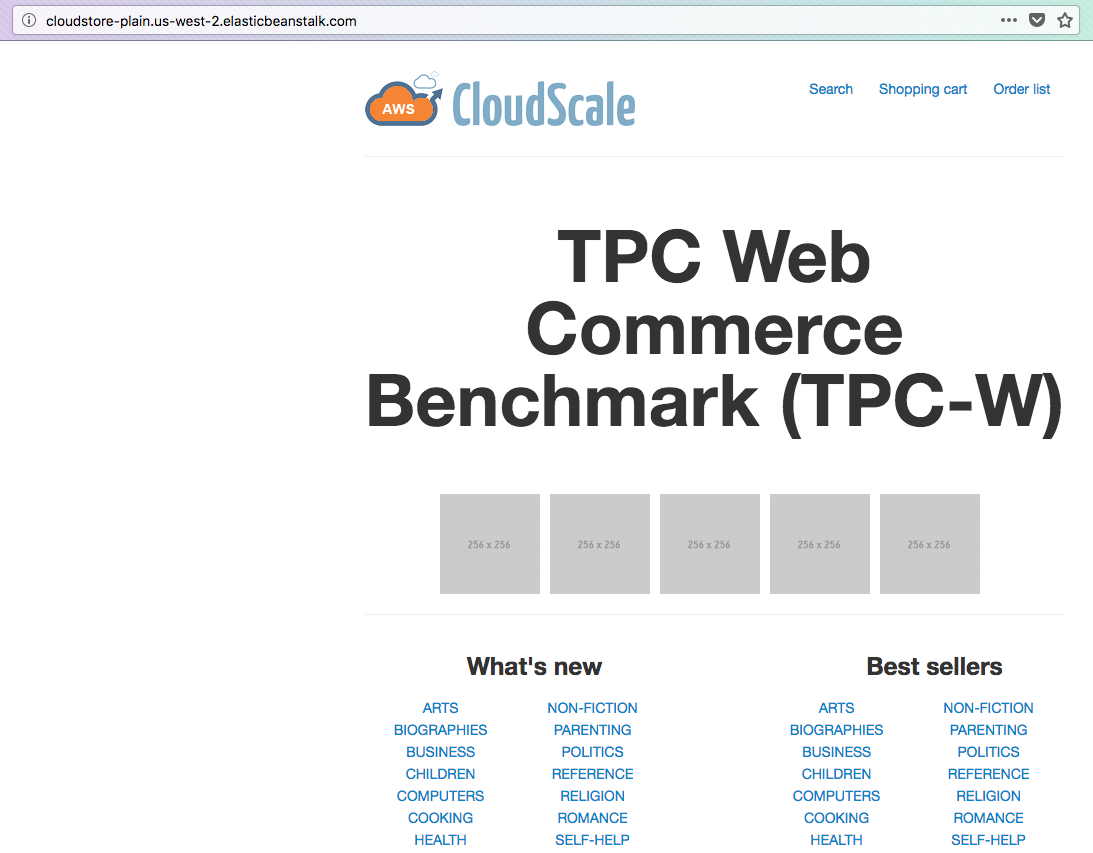
\includegraphics[width=14cm]{aws-cs-plain}
  \caption{\small{Versión original de \emph{CloudStore} (\emph{plain}) en AWS}}
  \label{fig:aws-cs-plain}
\end{figure}


\begin{figure}[h]
  \centering
  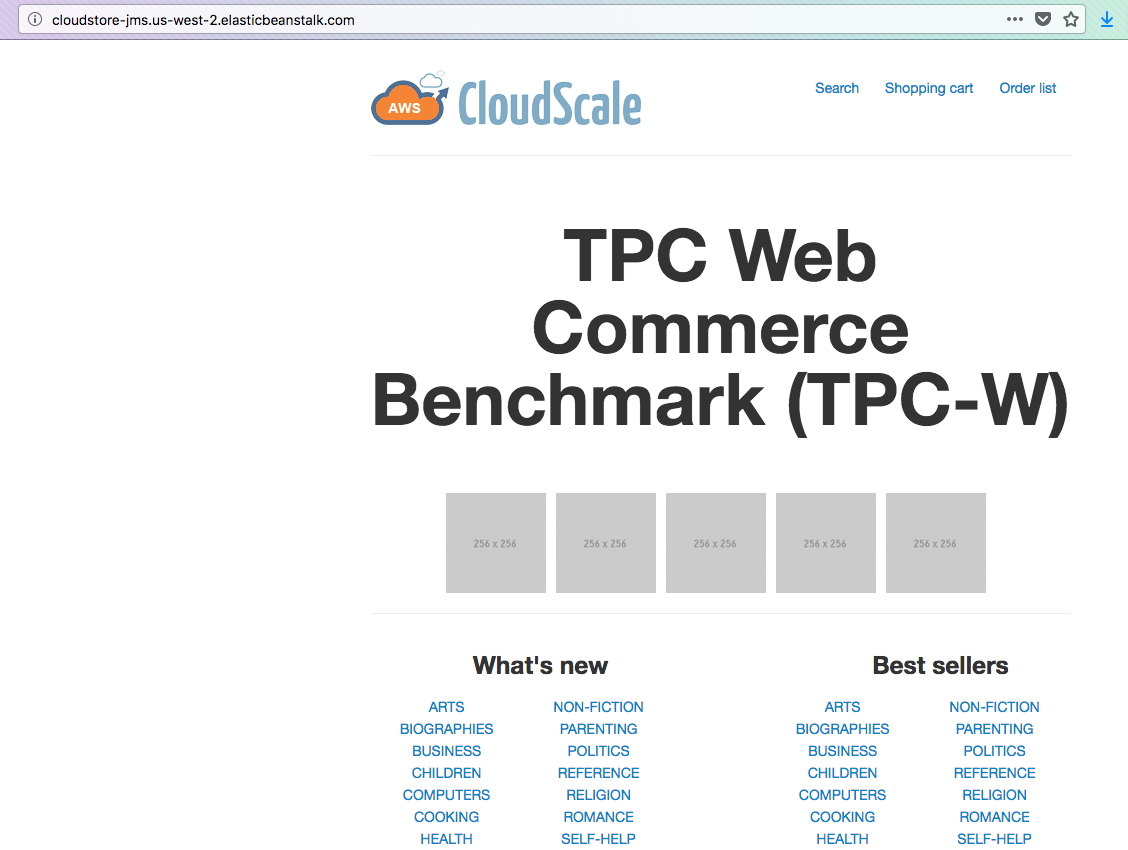
\includegraphics[width=14cm]{aws-cs-jms}
  \caption{\small{Versión de \emph{CloudStore} adaptada para MOM en AWS}}
  \label{fig:aws-cs-jms}
\end{figure}


\section{Mediciones de rendimiento iniciales} \label{ch:mediciones-iniciales}
Para realizar mediciones de rendimiento, los autores de \emph{CloudStore} crearon una herramienta de pruebas de carga basada en Apache JMeter\footnote{\url{https://jmeter.apache.org}} a la cual llamaron \emph{Distributed JMeter}. Esta herramienta se usa para crear cargas de trabajo las cual simulan múltiples usuarios realizando peticiones a un servidor Web el cual esté ejecutando \emph{CloudStore}. \emph{Distributed JMeter} se ejecuta en un entorno Linux en EC2 en AWS. Envía solicitudes \texttt{HTTP} a servicio de balanceo de carga \emph{Elastic Load Balancer}. JMeter registra los datos de todas las solicitudes y respuestas \texttt{HTTP}, lo que permite la medición de las característias del sistema tal y cómo el número de solicitudes que son exitosas, caducan o fallan. \emph{Distributed JMeter} se encuentra disponible en \url{https://github.com/CloudScale-Project/Distributed-Jmeter}. 

\begin{figure}[h]
  \centering
  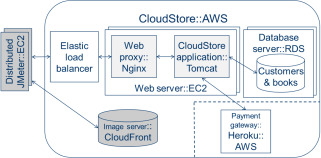
\includegraphics[width=10cm]{cloudstore-deployment}
  \caption{\small{Instalación de \emph{CloudStore} en AWS}}
  \label{fig:cs-deploy}
\end{figure}

En la figura \ref{fig:cs-deploy} se muestra la instalación de \emph{CloudStore} junto con el generador de pruebas de carga \emph{Distributed JMeter}, los componentes funcionales de \emph{CloudStore} (servidor Web, base de Datos, servidor de imágenes y \emph{gateway} de pagos) instalados en la platforma AWS.
\begin{itemize}
    \item El \emph{Elastic load balancer} es parte de AWS y es utilizado para distribuir tráfico entrante a la aplicación a través de múltiples instancias EC2. En la instalación de ambas versiones de \emph{CloudStore}, el servicio de balanceo se configura a través de \emph{Elastic BeanStalk}.
    \item Un servidor Web instalado en varias instancias EC2 que se ejecuta bajo un sistema operativo Linux y que consiste de dos componentes:
    \begin{enumerate}
        \item Un proxy Web basado en Nginx que reenvía peticiones \texttt{HTTP} a la aplicación de \emph{CloudStore}
        \item La aplicación de \emph{CloudStore}
    \end{enumerate}
    \item Un servidor de base datos que se proporciona a través de RDS y que ejecuta una base de datos MySQL.
    \item Para ambas versiones de \emph{CloudStore} se prescindió del servidor de imágenes que se propone en la instalación original de la figura \ref{fig:cs-deploy}. En su lugar, se modificó \emph{CloudStore} para que cada vez que se necesitara entregar una imagen, se entregara una por defecto
    \item Un \emph{gateway} de pagos, un generador simple de tiempos de respuesta que se introducido en lugar de un servicio de pagos externo. Con el fin de imitar un servicio real independiente a \emph{CloudStore}, el generador de tiempos de respuesta introduce un retraso definido a partir de una distribución estadística. El generador de tiempos de respuesta se instaló en una plataforma Heroku, la cual es completamente independiente a AWS. El repositorio de código para el generador de tiempos de respuesta se encuentra disponible en \url{https://github.com/CloudScale-Project/Response-Generator}
\end{itemize}
  

\subsection{Generación de cargas de trabajo con JMeter}
En \emph{Distributed JMeter} se ponen a disposición varias pruebas de carga para evaluar principalmente las características de escalabilidad de la aplicación (recordar que la aplicación \emph{CloudStore} fue creada validar los modelos y metodología de \emph{CloudScale}). Estas pruebas estan basadas en escenarios en donde miles de usuarios están accediendo de forma aleatoria a las diferentes páginas Web que componen \emph{CloudStore} por un tiempos de 10 - 15 minutos. A partir de esto, los autores esperan experimentar cambios el comportamiento de la aplicación debido al crecimiento/disminución en las instancias en donde se ejecuta.

Con el fin de explorar las características de \emph{CloudStore} y del impacto de agregar comunicación basada en mensajes para el procesamiento de pagos, se toma como referencia el escenario de prueba llamado \texttt{cloudscale-max} que se pone a disposición en \emph{Distributed JMeter}, en donde se simulan 2000 usuarios realizando peticiones a las páginas Web de \emph{CloudScale} durante 15 minutos de acuerdo a una distribución de probabilidades proporcionada dentro de la prueba. Se toma esta prueba como base y se modifica para utilizar 100 usuarios en lugar de 2000 y la duración de la se cambió a 2 - 3 minutos (La duración se cambió a 2 minutos, pero por lo general los hilos -\emph{threads} - de JMeter tienden a no finalizar luego del tiempo especificado). La intención detrás de esta modificación es la de explorar el comportamiento de \emph{CloudStore} a una escala la cual permita dar mejor seguimiento a las acciones que se dan a lo interno de la aplicación y de esta forma lograr tener un mejor entendimiento de la misma. También se busca, al contrario de los autores de \emph{CloudStore} no introducir cargas de trabajo que pudieran hacer que el ambiente de AWS cambiara porque esto podría impactar con los resultados de los tiempos de respuesta. 

\subsection{Pruebas sobre versión original de \emph{CloudStore}}
En la figura \ref{fig:jmeter-1} muestra JMeter configurado con la prueba \texttt{cloudscale-max}.
\begin{figure}[h]
  \centering
  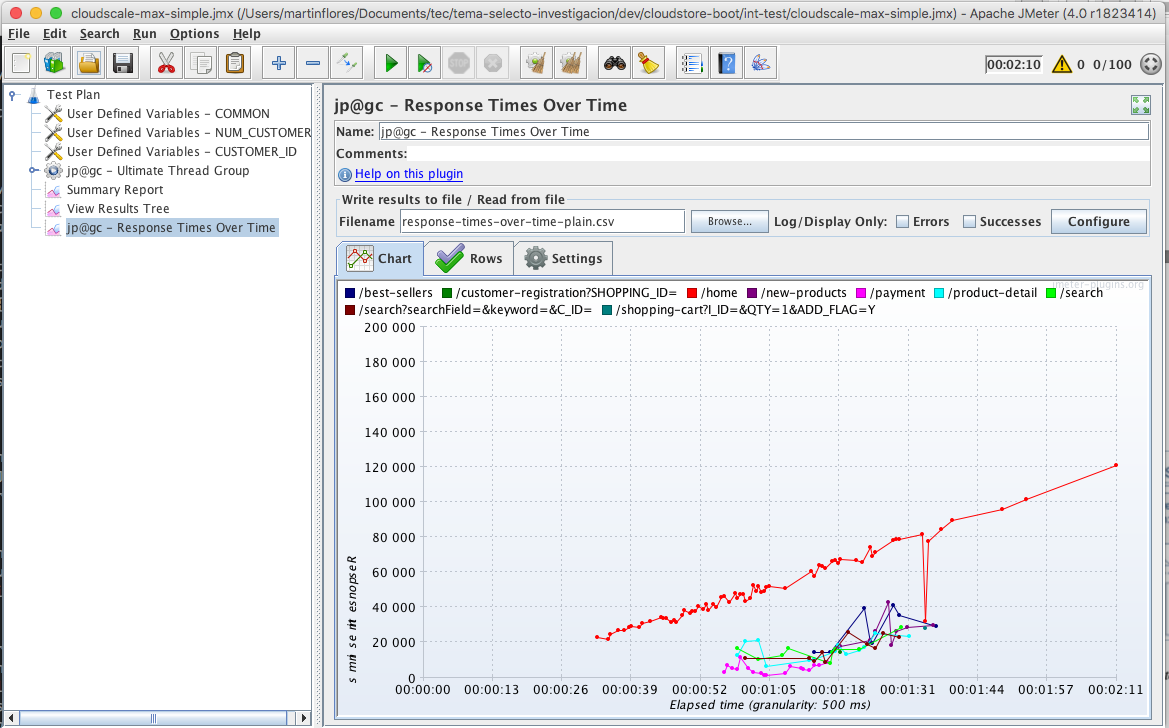
\includegraphics[width=13cm]{jmeter-1}
  \caption{\small{JMeter con la prueba \texttt{cloudscale-max}}}
  \label{fig:jmeter-1}
\end{figure}

Luego de ejecutar la prueba se pudo obtener los tiempos de respuesta sobre las páginas que componen la versión original de \emph{CloudStore}. En esta investigación se está particularmente interesado en la página(recurso Web) llamado \texttt{/payment} ya que es en este en donde se ejecut la lógica del pago, en dónde se realiza la conexión con el \emph{gateway} de pagos. En la figura \ref{fig:cs-plain-1} se muestran los resultados obtenidos. La línea de color fucsia es la que representa los tiempos de respuesta que experimentaron las solicitudes a \texttt{/payment}. Los resultados para \texttt{/payment} se pueden ver con mayor detalle en la figura \ref{fig:cs-plain-2}. 

\begin{figure}[h]
  \centering
  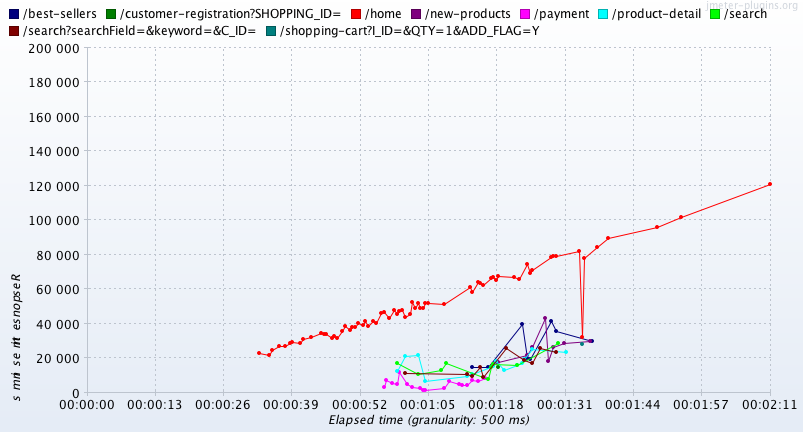
\includegraphics[width=15cm]{response-over-time-local-to-prod-1-plain}
  \caption{\small{Tiempos de respuesta de las páginas de la versión original \emph{CloudStore} (cloudstore-plain)}}
  \label{fig:cs-plain-1}
\end{figure}

\begin{figure}[h]
  \centering
  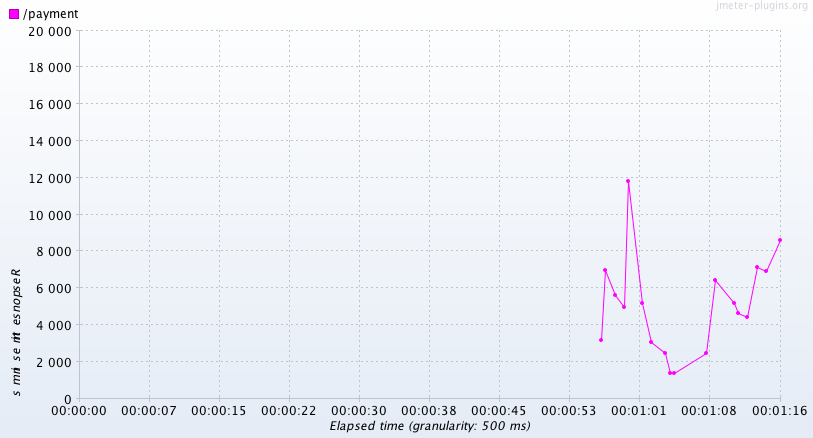
\includegraphics[width=15cm]{response-over-time-local-to-prod-1-plain-payment}
  \caption{\small{Tiempos de respuesta de \texttt{/payment} en la versión original de \emph{CloudStore}}}
  \label{fig:cs-plain-2}
\end{figure}

En promedio, las páginas Web de \emph{CloudStore} tomaron 30 segundos en ser servidas. La página de inicio, \texttt{/home}, representada en la línea roja de la figura \ref{fig:cs-plain-1} muestra un crecimiento sostenido desde el inicio hasta el fin de la prueba. La página de inicio realiza varios llamados a la base de datos con el fin de mostrar productos e información de la tienda, por lo que para esta página, la base de datos podría resultar el cuello de botella.

Con respecto a \texttt{/payment} (figura \ref{fig:cs-plain-2}), se obtuvieron tiempos de respuesta de 5 segundos en promedio. En la programación detrás de \texttt{/payment} solamente se lleva a cabo la invocación y conexión con el \emph{gateway} de pagos. En los resultados para \texttt{/payment} también se obtuvieron varios respuestas con código \texttt{503 - Service Unavailable}, lo que indica que en un ambiente de producción real, varias solicitudes de pago no pudieron ser atendidas debido a que el servidor Web o bien el \emph{gateway} de pagos no fueron capaces de procesar la solicitud.

Esta prueba se ejecutó desde la computadora personal del autor de esta investigación. Cabe mencionar de que cuando se ejecutó la misma prueba desde una máquina virtual en EC2 los tiempos de respuesta que se obtuvieron fueron alrededor de 40\% más rápido, las tendencias en cuanto al comportamiento de la aplicación se mantuvo similar.

\subsection{Pruebas sobre versión modificada de \emph{CloudStore}}
Se tomó la misma prueba, \texttt{cloudscale-max}, como referencia para esta prueba. Solamente se cambió el \emph{host} al cual apuntaba anteriormente para que realizara las pruebas sobre la versión modificada de \emph{CloudStore}.

Para la versión modificada de \emph{CloudStore} (figura \ref{fig:cs-jms-1}), el tiempo promedio de respuesta de una página es de 31 segundos. Se puede notar que el comportamiento de la aplicación se mantiene similar aunque sí se experimentan cambios sobre \texttt{/payment}.

\begin{figure}[h]
  \centering
  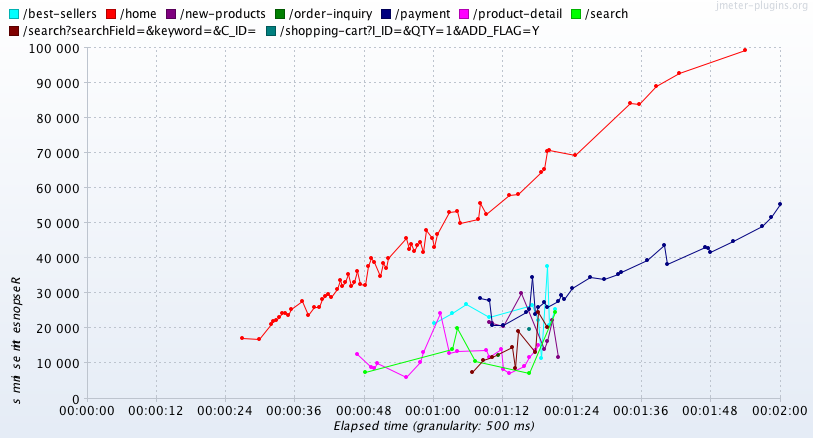
\includegraphics[width=15cm]{response-over-time-local-to-prod-1}
  \caption{\small{Tiempos de respuesta de las páginas de la versión modificada \emph{CloudStore} (cloudstore-jms)}}
  \label{fig:cs-jms-1}
\end{figure}

En la figura \ref{fig:cs-jms-2} se muestra el detalle de los tiempos de respuesta obtenidos en \texttt{/payment}. El tiempo de respuesta promedio de esta versión es de 35 segundos y mantuvo un crecimiento sostenido desde el inicio hasta el fin de la prueba. Este comportamiento es congruente con el comportamiento de la cola de mensajes: las solicitudes que tomaron menor tiempo fueron las que entraron de primero en la cola, las que duraron más fueron las que llegaron de último y por lo tanto fueron procesadas al final. Un dato interesante a tomar en cuenta es que en la versión modificada de \emph{CloudStore} el 100\% de las solitudes a \texttt{/payment} fueron exitosas, a diferencia de la versión original en donde se obtuvieron varias respuestas con código \texttt{503 - Service Unavailable}, principalmente hacia el final de la prueba. Esto sugiere que existen ocasiones en que el \emph{gateway} de pagos (el servicio generador de tiempos de respuesta) no puede manejar tantas solicitudes al mismo tiempo pero que cuando estas solicitudes se manejan por medio de comunicación basada en mensajes, cada solicitud de pago es servida adecuadamente. 

\begin{figure}[h]
  \centering
  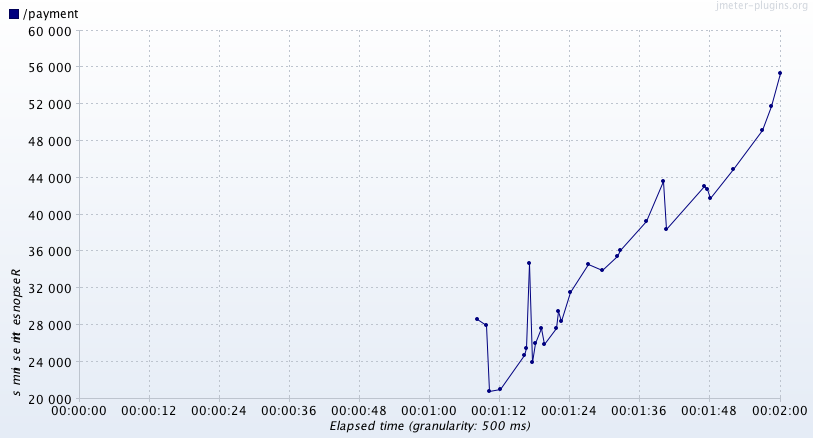
\includegraphics[width=15cm]{response-over-time-local-to-prod-1-payment}
  \caption{\small{Tiempos de respuesta de \texttt{/payment} en la versión modificada de \emph{CloudStore}}}
  \label{fig:cs-jms-2}
\end{figure}

En la prueba sobre la versión modificada de \emph{CloudStore}, solamente se puso a disposición un consumidor de mensajes, es decir, solamente una instancia de \texttt{jms-receiver} fue ejecutada. Cuando se ejecutaron varias instancias de \texttt{jms-receiver} al mismo tiempo, se experimentaron tiempos de respuesta más bajos. Cuando se probaron hasta 5 instancias al mismo tiempo, el tiempo bajó casi 50\%, y todas las solicitudes fueron exitosas. En la configuración original de \emph{CloudStore} este tipo de problemas se hubiera resulto por medio de la puesta en producción de más instancias.

El proyecto \emph{CloudScale} (del cual proviene \emph{CloudStore}) tiene su énfasis en modelado y rendimiento de escalabilidad, por lo que muchas de las pruebas que se incluyen en \emph{Distributed JMeter} están destinadas a estresar la infraestructuras para que estan puedan crecer y nuevas instancias de máquinas virtuales o bases de datos sean creadas. Luego de estas pruebas iniciales se considera que en \emph{CloudScale} también puede existir la oportunidad de evaluar el efecto que tiene en la escalabilidad el uso de comunicación basada en mensajes.

\subsection{Mediciones sobre máquina virtual que ejecuta ActiveMQ}
En la figura \ref{fig:aws-activemq-metrics} se muestran las métricas del uso del CPU y disco duro de la máquina virtual que estaba ejecutando ActiveMQ y el consumidor de mensajes (\texttt{jms-receiver}).

Durante la ejecución de la prueba de la sección anterior, la máquina virtual no experimentó operaciones de lectura/escritura en disco. Las colas de mensajes \texttt{payment-queue} y \texttt{payment-status-queue} no están configuradas para persistir datos y además \emph{CloudStore} delega almacenamiento y lectura de datos a la base de datos MySQL. En cuanto al uso del CPU, la máquina virtual experimentó un incremento de 0.5\% del uso del CPU durante la ejecución de la prueba. 

\begin{figure}[h]
  \centering
  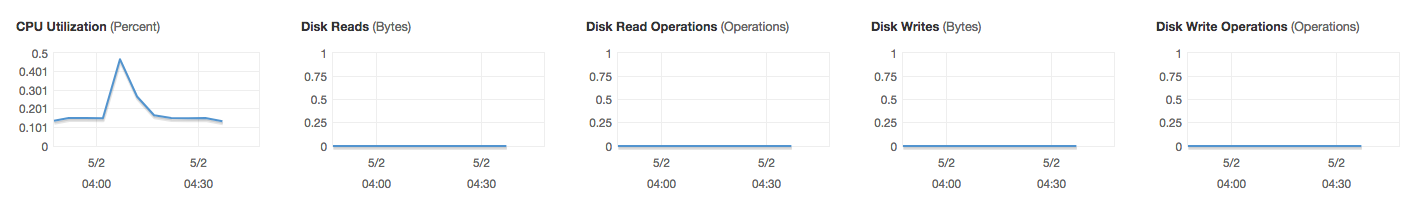
\includegraphics[width=18cm]{aws-activemq-metrics}
  \caption{\small{Métricas del rendimiento de la máquina virtual que ejecuta ActiveMQ en EC2}}
  \label{fig:aws-activemq-metrics}
\end{figure}

\section{Trabajo Futuro}
Las mediciones que se presentan en este informe se hicieron con el fin de empezar a probar y conocer cómo se comporta la aplicación de referencia. En las próximas semanas se pretende seguir experimentando con estas y otras mediciones con el fin de identificar características relevantes que puedan servir de entrada para el modelo de la aplicación y su posterior simulación.

Tal y como se mencionó en la sección \ref{ch:aplicacion-referencia}, una de las principales características por la cual se escogió \emph{CloudStore} como aplicación de referencia, es porque para esta aplicación ya se cuenta con un modelo basado en Palladio. Este modelo fue realizado por los autores de \emph{CloudStore} y se encuentra en el repositorio de código del mismo en GitHub. En este modelo se incluyen experimentos, los cuales son pruebas de carga que el \emph{Palladio Workbench} utiliza para simular el uso que le podrían dar los usuarios. 

Para las próximas semanas, se pretende empezar a trabajar con el \emph{Palladio Workbench} y el modelo de \emph{CloudStore}. Ejecutar experimentos/pruebas y evaluar resultados. Luego se agregarán nuevos componentes a este modelo: estos componentes serán los que representen el \emph{middleware} orientado a mensajes y la aplicación consumidora de mensajes. En esta parte, artículos que se han recopilado sobre el tema y las mediciones hechas servirán como entrada para modelar estos componentes.

Por último, se ejecutarán simulaciones sobre el modelo modificado y se compararán las métricas obtenidas con las que se han obtenido cuando se utilizó JMeter para probar \emph{CloudStore}. En este punto intentará saber si el modelo propuesto es uno que puede describir bien el comportamiento de esta aplicación.

\chapter{Propuesta de contenidos de informe final} \label{ch:propuesta-informe}
Los siguientes son los contenidos que se proponen para el informe final:
\begin{enumerate}
    \item Resumen (\emph{Abstract})
    \item Introducción: generalidades de los temas que se van a cubrir así como de la estructura del artículo
    \item Ingeniería de rendimiento de software:
    \begin{enumerate}
        \item Ingeniería de rendimiento a través de modelado
        \item Modelado de Arquitecturas de Software con el \emph{Palladio Component Model} (PCM)
    \end{enumerate}
    \item \emph{Middleware} Orientado a Mensajes: resumen de sección \ref{sec:mom}
    \item Modelado de rendimiento en una aplicación: \emph{CloudStore}
    \begin{enumerate}
        \item Generalidades de \emph{CloudStore}
        \item \emph{CloudStore} con \emph{middleware} orientado a mensajes
        \item Modelado de \emph{middleware} orientado a mensajes en \emph{CloudStore}
    \end{enumerate}
    \item Resultados: dar a conocer los resultados de las simulaciones sobre el modelo de \emph{CloudStore} y si los mismos logran predecir de alguna forma el comportamiento de la aplicación
    \item Trabajos Relacionados
    \item Conclusión
    \item Bibliografía
\end{enumerate}



%\chapter{Objetivos}
%
%\section{Objetivo General}
%%Diseñar un modelo de sistemas distribuidos de intercambio mensajes (\emph{message-oriented middleware}) para evaluar la influencia que tienen en el rendimiento de un sistema de software por medio de modelado y simulación basado en componentes.
%
%Diseñar un método para modelar sistemas distribuidos de intercambio de mensajes (\emph{message-oriented middleware}) para evaluar la influencia que tienen en el rendimiento de un sistema de software.
%
%\section{Objetivos Específicos}
%\begin{enumerate}
%    \item \label{itm:obj1}Revisión del estado del arte de trabajos relacionados con enfoques de predicción y medición del rendimiento en sistemas de software basados en componentes y en \emph{middleware} orientado a mensajes
%    \item \label{itm:obj2}Adaptar un sistema de software de referencia para el cual ya exista un modelo de rendimiento y simulaciones para que se integre y comunique con \emph{middleware} orientado a mensajes.
%    \item \label{itm:obj3}Comparar la solución implementada bajo diferentes cargas de trabajo
%    \item \label{itm:obj4}Crear un modelo del nuevo sistema y su rendimiento 
%    \item \label{itm:obj5}Validar y analizar el modelo creado a través de experimentos
%\end{enumerate}

%\chapter{Entregables}
%
%\section{Revisión de literatura}
%\paragraph{Alineado con objetivo específico~\ref{itm:obj1}}
%
%\paragraph{} Se pretende identificar los resultados de otros estudios relacionados con modelaje de rendimiento de software, así como retos y oportunidades de investigación que existan en esta área. Las preguntas de investigación inicialmente propuestas para conducir esta revisión son las siguientes:
%\begin{enumerate}
%    \item[\textbf{PI1}] ¿Cuáles enfoques de predicción y medición del rendimiento en sistemas de software basados en componente se han propuesto?
%    \item[\textbf{PI2}] ¿Cuáles enfoques de predicción y medición de rendimiento de software se han utilizado para \emph{middleware} orientado a mensajes?    
%    \item[\textbf{PI3}] ¿Qué retos y oportunidades existen con estos enfoques en la actualidad?
%    \item[\textbf{PI4}] ¿Qué herramientas hay disponibles para modelaje de rendimiento de software?
%\end{enumerate}


%\section{Aplicación adaptada para que soporte comunicación basada en mensajes}
%\paragraph{Alineado con objetivos específicos~\ref{itm:obj2} y \ref{itm:obj3}}  
%
%\paragraph{}Una vez que se haya identificado un sistema de software del cual ya exista un modelo de rendimiento y simulaciones, este se tomará como base para adaptarlo de tal forma que utilice \emph{middleware} orientado a mensajes en algún punto de su ejecución.
%
%A la aplicación adaptada se le realizarán mediciones de su rendimiento con el fin de tener estos como entrada para las subsecuentes tareas de modelado propuestas. Serán estas mediciones las que ayudan a refinar y calibrar el modelo.
%
%\section{Modelo de rendimiento del nuevo sistema}
%\paragraph{Alineado con objetivos específicos~\ref{itm:obj4} y \ref{itm:obj5}}
%
%\paragraph{}A partir del sistema adaptado y sus mediciones, se modificará el modelo de rendimiento original del sistema de referencia para reflejar los cambios introducidos por el \emph{middleware} orientado a mensajes.
%
%Este nuevo modelo se ejercitará con los perfiles de uso de la aplicación de referencia, con el fin de validar si este puede aproximar el comportamiento del sistema ahora que se le han introducido cambios. 
%
%\chapter{Cronograma}
%Se cuentan con aproximadamente 11 semanas para llevar a cabo este trabajo. Las primeras dos semanas se van a dedicar a hacer una revisión de la literatura relevante. 
%
%Luego de esto, se dedicarán cuatro semanas a seleccionar una aplicación de referencia y adaptarla para que utilice comunicación basada en mensajes en algún punto de su ejecución. Una vez adaptada se ejecutarán pruebas de carga para determinar cuál es su rendimiento. 
%
%La última etapa de la investigación será la de crear un modelo del rendimiento del nuevo sistema utilizando PCM. A este modelo se le ejecutarán simulaciones de uso con el fin de ir calibrando su precisión.
%
%A continuación se presenta el calendario de actividades propuesto para esta investigación: 
%
%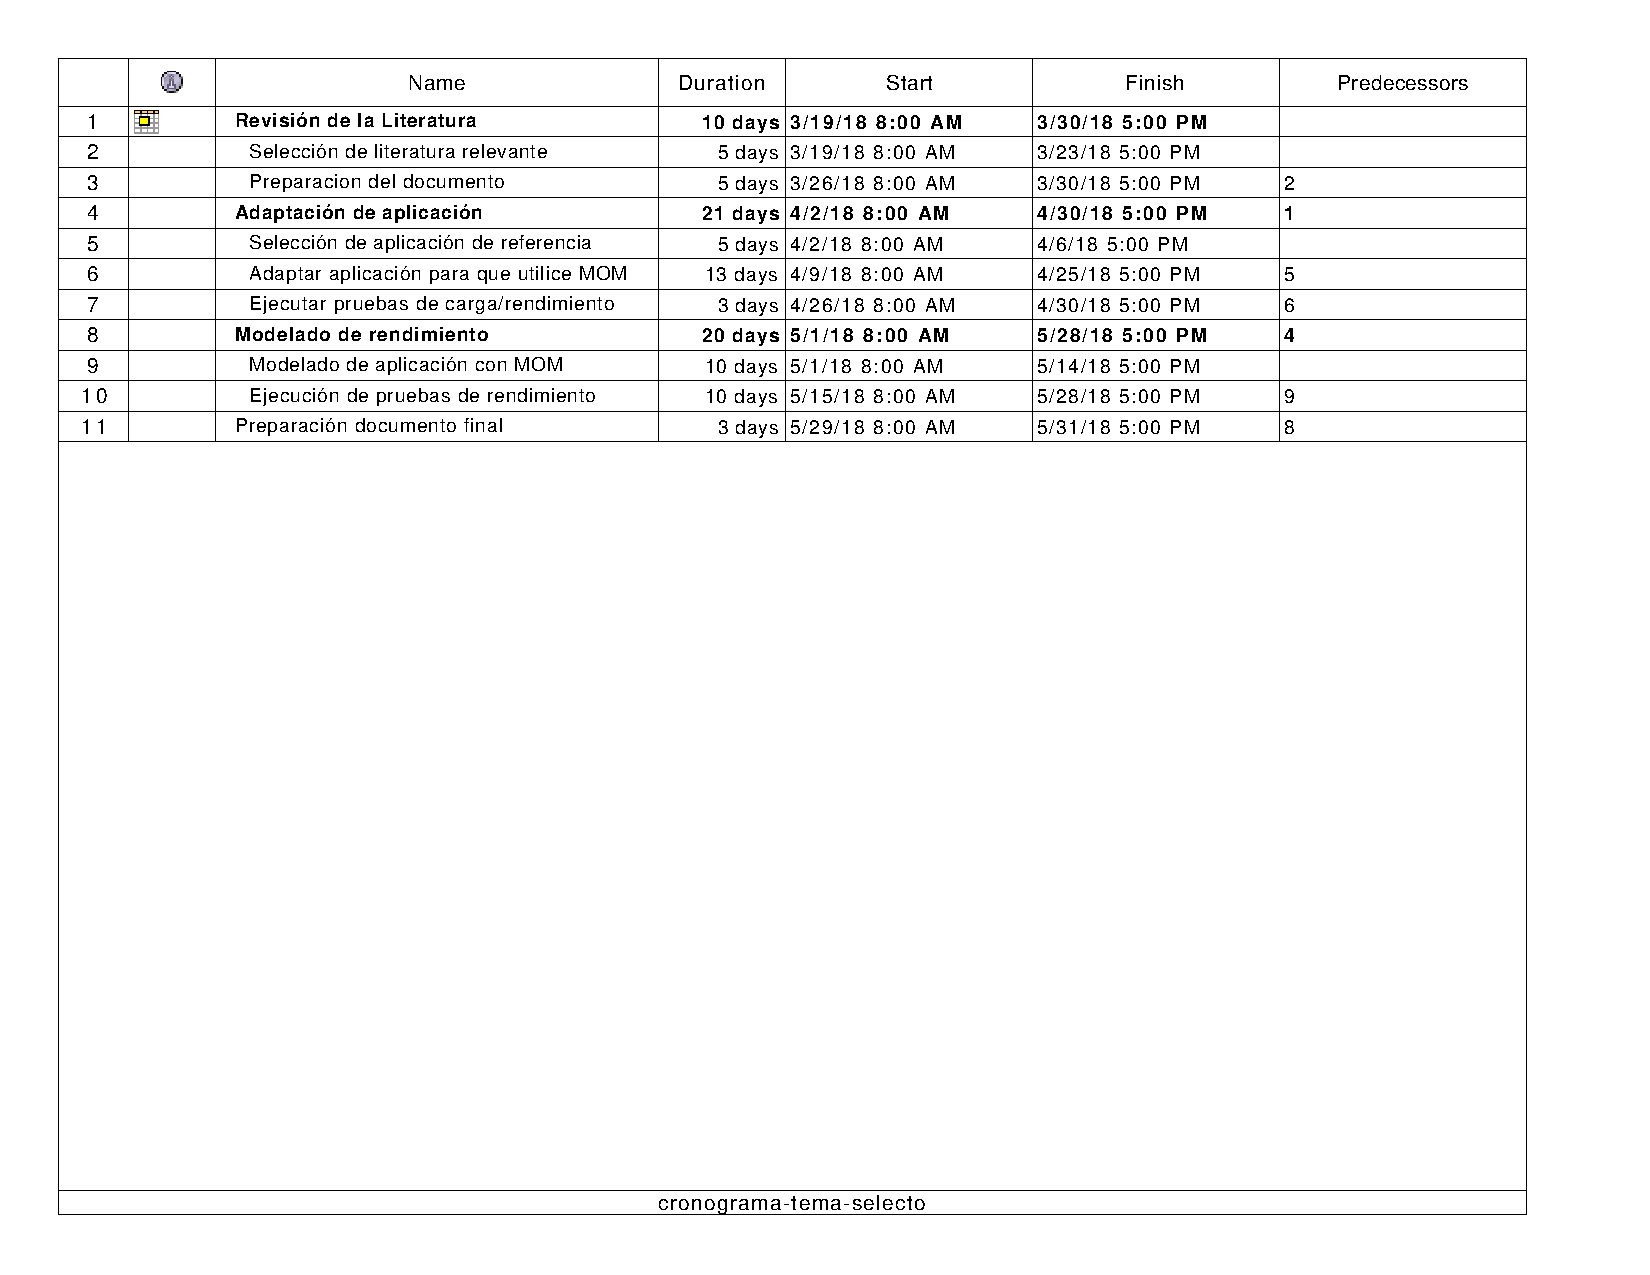
\includepdf[landscape, pages=1]{cronograma-tema-selecto-1}
%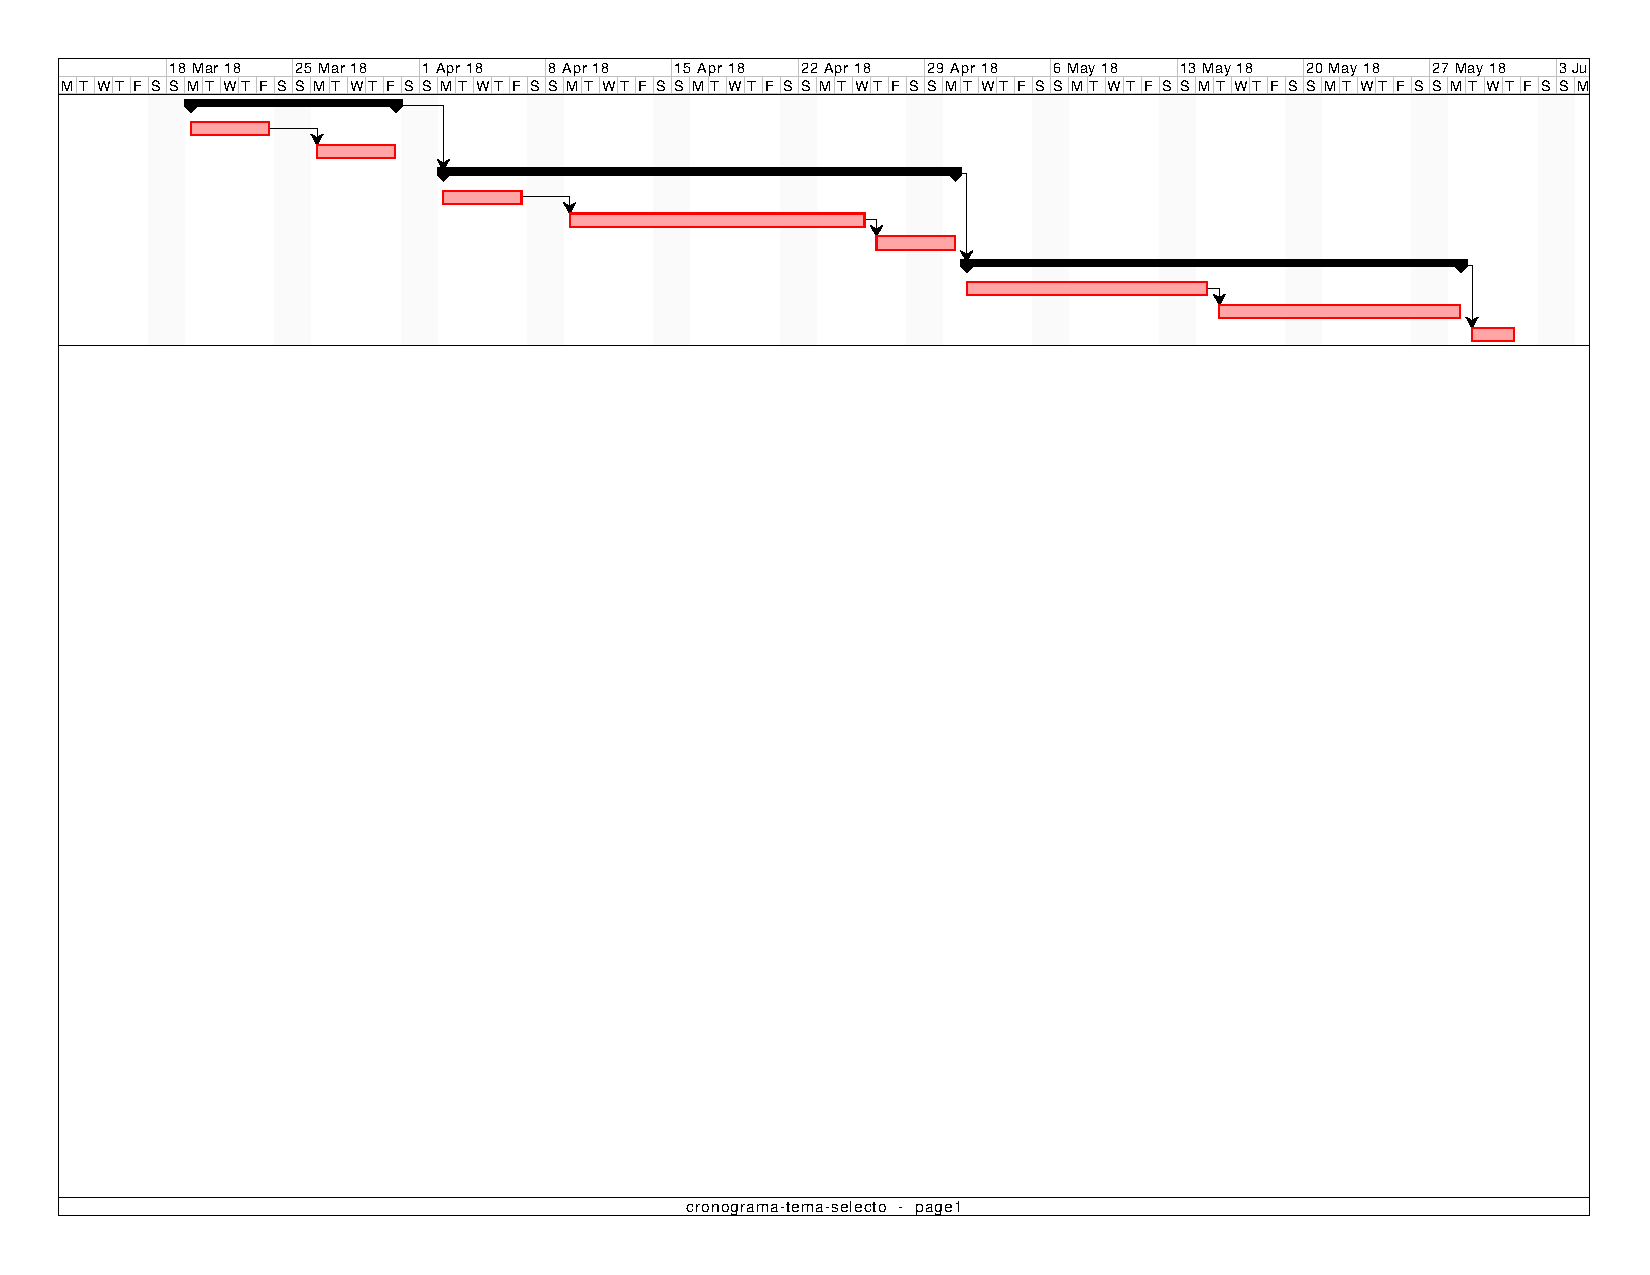
\includepdf[landscape, pages=1]{cronograma-tema-selecto-2}

\addcontentsline{toc}{chapter}{Bibliografía}
\bibliographystyle{ACM-Reference-Format}
\begin{thebibliography}{9}

\bibitem{palladio-blue-book} Ralf H. Reussner, Steffen Becker, Jens Happe, Robert Heinrich, Anne Koziolek, Heiko Koziolek, Max Kramer, and Klaus Krogmann. \emph{Modeling and Simulating Software Architectures: The Palladio Approach}. The MIT Press. 2016.

\bibitem{activemq-in-action} Bruce Snyder, Dejan Bosnanac, Rob Davies. \emph{ActiveMQ in Action}. Manning, 2011.

\bibitem{alwakeel} S.S. Alwakeel and H.M. Almansour. \emph{Modeling and Performance Evaluation of Message-oriented Middleware with Priority Queuing}. Information Technology Journal, 10: 61-70. 2011. DOI \url{http://dx.doi.org/10.3923/itj.2011.61.70}

\bibitem{chew} Chew, Zen Bob. \emph{Modelling Message-oriented-middleware Brokers Using Autoregressive Models for Bottleneck Prediction}. PhD Thesis. Queen Mary, University of London. 2013. \url{https://qmro.qmul.ac.uk/jspui/handle/123456789/8832}

\bibitem{liu-gordon} Yan Liu and Ian Gorton. \emph{Performance prediction of J2EE applications using messaging protocols}. In Proceedings of the 8th international conference on Component-Based Software Engineering (CBSE'05), George T. Heineman, Ivica Crnkovic, Heinz W. Schmidt, Judith A. Stafford, and Clemens Szyperski (Eds.). Springer-Verlag, Berlin, Heidelberg, 1-16. 2005. DOI \url{http://ezproxy.itcr.ac.cr:2075/10.1007/11424529_1} 

\bibitem{microservices-challenges} Robert Heinrich, André van Hoorn, Holger Knoche, Fei Li, Lucy Ellen Lwakatare, Claus Pahl, Stefan Schulte, and Johannes Wettinger. \emph{Performance engineering for microservices: Research challenges and directions}. In Companion Proceedings of the 8th ACM/SPEC on International Conference on Performance Engineering, 2017, pages 223-226. DOI: \url{https://doi.org/10.1145/3053600.3053653}

\bibitem{performance-devops} Andreas Brunnert, André van Hoorn, Felix Willnecker, Alexandru Danciu, Wilhelm Hasselbring, Christoph Heger, Nikolas Roman Herbst, Pooyan Jamshidi, Reiner Jung, Jóakim von Kistowski, Anne Koziolek, Johannes Kroß, Simon Spinner, Christian Vögele, Jürgen Walter, and Alexander Wert. \emph{Performance-oriented devops: A research agenda}. Technical Report SPEC-RG-2015-01, SPEC Research Group - DevOps Performance Working Group, Standard Performance Evaluation Corporation (SPEC), 2015. \url{http://arxiv.org/abs/1508.04752}

\bibitem{martince-et-al} Tomáş Martinec, Lukáş Marek, Antonín Steinhauser, Petr Tůma, Qais Noorshams, Andreas Rentschler, and Ralf Reussner. \emph{Constructing performance model of JMS middleware platform}. In Proceedings of the 5th ACM/SPEC international conference on Performance engineering (ICPE '14). ACM, New York, NY, USA, 123-134. 2014. DOI: \url{https://ezproxy.itcr.ac.cr:2878/10.1145/2568088.2568096}

\bibitem{jms20} Mark Richards, Richard Monson-Haefel, David Chappell. \emph{Java Message Service}. O'Reilly Media. Segunda Edición. 2009.

\bibitem{huber-et-al} Nikolaus Huber, Steffen Becker, Christoph Rathfelder, Jochen Schweflinghaus, and Ralf H. Reussner. 2010. \emph{Performance modeling in industry: a case study on storage virtualization}. In Proceedings of the 32nd ACM/IEEE International Conference on Software Engineering - Volume 2 (ICSE '10), Vol. 2. ACM, New York, NY, USA, 1-10. DOI: \url{http://ezproxy.itcr.ac.cr:2075/10.1145/1810295.1810297} 

\bibitem{palladio-seminal} Stephen Becker, Heiko Koziolek and Ralf Reussner. \emph{The Palladio component model for model-driven prediction}. Journal of Systems and Software 82:3-22. Elsevier Science Inc. 2009. DOI: \url{http://dx.doi.org/10.1016/j.jss.2008.03.066}

\bibitem{noorshams} Qais Noorshams. \emph{Modeling and Prediction of I/O Performance in Virtualized Environments}. PhD thesis, Karlsruhe Institute of Technology (KIT), 2015. URL: \url{http://digbib.ubka.uni-karlsruhe.de/volltexte/1000046750}


\bibitem{happe-et-al} Jens Happe, Holger Friedrich, Steffen Becker, and Ralf H. Reussner. \emph{A pattern-based performance completion for Message-oriented Middleware}. In Proceedings of the 7th international workshop on Software and performance (WOSP '08). ACM, New York, NY, USA, 165-176. 2008. DOI: \url{http://ezproxy.itcr.ac.cr:2075/10.1145/1383559.1383581} 


\bibitem{performance-model-survey} Heiko Koziolek. 2010. \emph{Performance evaluation of component-based software systems: A survey. Perform}. Eval. 67, 8 (August 2010), 634-658. DOI: \url{http://ezproxy.itcr.ac.cr:2075/10.1016/j.peva.2009.07.007} 

\bibitem{case-study-1} Thijmen de Gooijer, Anton Jansen, Heiko Koziolek, and Anne Koziolek. 2012. \emph{An industrial case study of performance and cost design space exploration}. In Proceedings of the 3rd ACM/SPEC International Conference on Performance Engineering (ICPE '12). ACM, New York, NY, USA, 205-216. DOI: \url{https://ezproxy.itcr.ac.cr:2878/10.1145/2188286.2188319}

\bibitem{rathfelder-et-al} Christoph Rathfelder, Steffen Becker, Klaus Krogmann and Ralf Reussner. \emph{Workload-aware System Monitoring Using Performance Predictions Applied to a Large-scale E-Mail System}. 2012 Joint Working IEEE/IFIP Conference on Software Architecture and European Conference on Software Architecture, Helsinki, 2012, pp. 31-40.
DOI: \href{https://ezproxy.itcr.ac.cr:2878/10.1109/WICSA-ECSA.212.11}{10.1109/WICSA-ECSA.212.11}. 

\bibitem{media-store} Misha Strittmatter and Amine Kechaou. \emph{The media store 3 case study system}. Technical Report 2016,1, Faculty of Informatics, Karlsruhe Institute of Technology, 2016. URL: \url{http://digbib.ubka.uni-karlsruhe.de/volltexte/documents/3792054}

\bibitem{woodside-et-al} Murray Woodside, Greg Franks, and Dorina C. Petriu. \emph{The Future of Software Performance Engineering}. Future of Software Engineering (FOSE '07), pages 171-187, May 2007. DOI 10.1109/FOSE.2007.32

\bibitem{thijmen-thesis} Thijmen de Gooijer. \emph{Performance Modeling of ASP.Net Web
Service Applications: an Industrial Case Study}. Master's thesis, Malardalen University, Vasteras, Sweden, 2011.

\bibitem{palladion-screencast} Steffen Becker. \emph{Palladio-Bench Screencasts}. \url{http://www.
palladio-simulator.com/tools/screencasts/} Accesado el 20 de Marzo del 2018.

\bibitem{jit-et-al} Yan Jin, Antony Tang, Jun Han, and Yan Liu. \emph{Performance Evaluation and Prediction for Legacy Information Systems}. 29th International Conference on Software Engineering (ICSE'07), pages 540-549, May 2007.

\bibitem{balsamo-et-al} Simonetta Balsamo, Antinisca DiMarco, Paola Inverardi, and Marta
Simeoni. \emph{Model-based performance prediction in software development: A survey}. IEEE Trans. Softw. Eng., 30(5):295–310, May 2004.

\bibitem{peropteryx} Anne Koziolek, Heiko Koziolek, and Ralf Reussner. \emph{PerOpteryx: automated application of tactics in multi-objective software architecture optimization}. In Proceedings of the joint ACM SIGSOFT conference -- QoSA and ACM SIGSOFT symposium -- ISARCS on Quality of software architectures -- QoSA and architecting critical systems -- ISARCS (QoSA-ISARCS '11). ACM, New York, NY, USA, 33-42. 2011. DOI=\url{http://ezproxy.itcr.ac.cr:2075/10.1145/2000259.2000267}

\bibitem{descartesml} Samuel Kounev and Fabian Brosig and Nikolaus Huber. \emph{The Descartes Modeling Language}. Technical Report. Department of Computer Science, University of Wuerzburg. 2014.
%
%\bibitem{cloudscale} Sebastian Lehrig and Steffen Becker. 2015. \emph{The CloudScale Method for Software Scalability, Elasticity, and Efficiency Engineering: a Tutorial}. In Proceedings of the 6th ACM/SPEC International Conference on Performance Engineering (ICPE '15). ACM, New York, NY, USA, 329-331. 2015. DOI: \url{https://ezproxy.itcr.ac.cr:2878/10.1145/2668930.2688818}

\bibitem{cloudscale} Gunnar Brataas, Erlend Stav, Sebastian Lehrig, Steffen Becker, Goran Kopčak, and Darko Huljenic. 2013. \emph{CloudScale: scalability management for cloud systems}. In Proceedings of the 4th ACM/SPEC International Conference on Performance Engineering (ICPE '13), Seetharami Seelam (Ed.). ACM, New York, NY, USA, 335-338. 2013. DOI: \url{https://ezproxy.itcr.ac.cr:2878/10.1145/2479871.2479920}

\bibitem{spe-ed} Connie U Smith and Lloyd G Williams. \emph{Performance solutions: a practical guide to creating responsive, scalable software}. Addison Wesley Longman Publishing Co., Inc., Redwood City, CA, USA, 2002.

\bibitem{woodside-et-al-2} Murray Woodside, Dorin Petriu, and Khalid Siddiqui. \emph{Performance-related Completions for Software Specifications}. In Proceedings of the 24th International Conference on Software Engineering, pages 22–32, New York, NY, USA, 2002.

\end{thebibliography}







%\addcontentsline{toc}{chapter}{Resumen}
%\chapter*{Resumen}
%A pesar de la popularidad de las metodologías ágiles de desarrollo de software en la industria, expresada en varias encuestas y estudios recientes, muchas organizaciones siguen reportando en estas mismas encuestas que se cuenta con poco personal capacitado con las habilidades necesarias y que los planes de estudio de carreras de tecnología de información muestran rezagos en estos temas. Con el fin de brindar una formación que no solamente incluya la enseñanza de prácticas ágiles sino también el desarrollo de otras actitudes como el trabajo en equipo y el empredurismo, las universidades han venido introduciendo paulativamente estas prácticas a sus planes de estudio principalmente por medio de enfoques de \emph{aprender-haciendo}. Universidades en Costa Rica también han reportado la inclusión de estos temas en sus planes de estudio como respuesta a las tendencias mundiales y para apoyar la creciente industria de desarrollo de software del país.
%
%
%\addcontentsline{toc}{section}{\emph{Abstract}}
%\section*{\emph{Abstract}}
%Despite the popularity of the agile engineering practices in the software industry reported in recent surveys and studies, many organizations keep reporting in those same surveys which they have no enough personal with the desired skill set, and also that they think that IT curricula is behind in these new software development trends. In order to provide an education which involves agile engineering practices but also other skills such as teamwork and entrepreneurship, universities have been introducing these practices in their curricula, mainly by the use of \emph{learning-by-doing} approaches. Universities in Costa Rica have reported the introduction of these topics in their curricula as a response to their increasing popularity and to support the growing software industry in the country.  
%
%\addcontentsline{toc}{section}{\emph{Palabras Clave / Keywords}}
%\subsection*{Palabras Clave / Keywords}
%agile software development, agile teaching, agile engieering practices, software engineering education, costa rica software education


%%%%%%%%%%%%%
% Capitulos %

%\chapter*{Introducción}
%\pagenumbering{arabic}
%\addcontentsline{toc}{chapter}{Introducción}
%\input{capitulos/introduccion}
%
%\chapter{Generalidades de la Investigación}
%\input{capitulos/ch1}
%
%\chapter{Marco Teórico} \label{ch2:marco-teorico}
%\input{capitulos/ch2}
%
%\chapter{Marco Metodológico}
%\input{capitulos/ch3}
%
%
%\chapter{Resultados Esperados}
%\input{capitulos/ch4}
%
%\chapter{Plan de Trabajo}
%\input{capitulos/ch5}
%
%% Bibliografia
%\addcontentsline{toc}{chapter}{Bibliografía}
%\input{capitulos/bibliografia}
%
%\addcontentsline{toc}{chapter}{Apéndice}
%\chapter*{Apéndice}
%\input{capitulos/apendice}

%Portada
% 
% 
%\frontmatter
% 
%\addcontentsline{toc}{chapter}{Forewordq}
%hola
% 
%\addcontentsline{toc}{chapter}{Dummy entry}
%Some text...
% 
%\tableofcontents
% 
%\mainmatter
% 
%\chapter{First Chapter}
% 
%This will be an empty chapter...
 
\end{document}

